%% -----------------------------------------------------------------
%% This file uses UTF-8 encoding
%%
%% For compilation use following command:
%% latexmk -pdf -pvc -bibtex --shell-escape thesis
%%
%% -----------------------------------------------------------------
%%                                     _     _      
%%      _ __  _ __ ___  __ _ _ __ ___ | |__ | | ___ 
%%     | '_ \| '__/ _ \/ _` | '_ ` _ \| '_ \| |/ _ \
%%     | |_) | | |  __/ (_| | | | | | | |_) | |  __/
%%     | .__/|_|  \___|\__,_|_| |_| |_|_.__/|_|\___|
%%     |_|                                          
%%
%% -----------------------------------------------------------------

\documentclass{kithesis}

% Additional packages
\usepackage[english,slovak]{babel}
\usepackage{blindtext}  % lorem ipsum
\usepackage{amssymb}
\usepackage{tikz}
%\usepackage{minted}

\newcommand*{\field}[1]{\mathbb{#1}}%
\usetikzlibrary{calc}
\usepackage{tkz-euclide}
\usetkzobj{all}
\usepackage{braket}

% Variables
%\thesisspec{figures/thesisspec.png} 

\title{Measurement and interaction of quantum circutis}{Meranie a interakcia kvantových obvodov}

\author{Marián Sabat}
\supervisor{prof. Ing. Ján Kollár, CSc.} %veduci prace
%\consultant{Donald E. Knuth} %konzultant
\college{Techincal University of Kosice}{Technicka Univerzita v Kosiciach} %univerzita
\faculty{Faculty of Electrical Engineering and informatics}{Fakulta elektrotechniky a informatiky} %fakulta
\department{Department of Computers and Informatics}{Katedra počítačov a informatiky} %katedra
\departmentacr{DCI}{KPI} % skratka katedry
\thesis{Master thesis}{Diplomová práca} %typ prace
\submissiondate{1}{1}{2020}
\fieldofstudy{9.2.1 Informatika}
\studyprogramme{Informatika}
%\city{Košice} %mesto
\keywords{Quantum comuters and other key words}{Kvantove pocitace a ine klucove slova}

\declaration{Vyhlasujem, ze vsetko som pisal sam ...}

\abstract{
    % english 
	%\blindtext
	ABSTRAKT
}{
    % slovak 
	%\blindtext
	ABSTRAKT
}

\acknowledgment{%Na tomto mieste by som rád poďakoval svojmu vedúcemu práce za jeho čas a odborné vedenie počas riešenia mojej záverečnej práce.

%Rovnako by som sa rád poďakoval svojim rodičom a priateľom za ich podporu a povzbudzovanie počas celého môjho štúdia.
    
%V neposlednom rade by som sa rád poďakoval pánom {\it Donaldovi E. Knuthovi} a {\it Leslie Lamportovi} za typografický systém \LaTeX, s ktorým som strávil množstvo nezabudnuteľných večerov.
}

\addbibresource{chapters/bibliography.bib}

% if you want to work only on selected chapters
%\includeonly{chapters/analyza} %,chapters/synteza}

% Load acronyms
\newacronym{ny}{NY}{New York}
\newacronym{la}{LA}{Los Angeles}
\newacronym{un}{UN}{United Nations}
\newacronym{gcd}{GCD}{Greatest Common Divisor}
\newacronym{lcm}{LCM}{Least Common Multiple}


%% -----------------------------------------------------------------
%%          _                                       _   
%%       __| | ___   ___ _   _ _ __ ___   ___ _ __ | |_ 
%%      / _` |/ _ \ / __| | | | '_ ` _ \ / _ \ '_ \| __|
%%     | (_| | (_) | (__| |_| | | | | | |  __/ | | | |_ 
%%      \__,_|\___/ \___|\__,_|_| |_| |_|\___|_| |_|\__|
%%                                                      
%% -----------------------------------------------------------------

\begin{document}
%% Title page, abstract, declaration etc.:
\frontmatter{}

%% List of code listings, if you are using package minted
%\listoflistings

\pagenumbering{arabic}

%% Chapters
% !TEX root = ../thesis.tex

\chaptermark{Úvod}
\addcontentsline{toc}{chapter}{Úvod}

\chapter*{Úvod}

Systémy, ktoré sa dokážu učiť z dát sú už dnes prístupné verejnosti. Je čoraz jednoduchšie študovať techniky strojového učenia a preto progres v tomto odvetví je skutočne viditeľný. Množstvo dát a dobrá výpočtová technika majú za následok, že v takmer všetkých oblastiach sa zavádza nejaký druh umelej inteligencie. Počítače, ktoré by rozumeli informáciám by znamenali revolúciu v našich životoch. Program, ktorý by dokázal vygenerovať obraz na základe hudobného podkladu, na základe emócií a nálad, ktoré sú obsiahnuté v hudbe by bol pokrok ku umelej inteligencii, ktorá by skutočne rozumela dátam.

Proces syntézy jedného druhu informácií na iní je pre ľudí prirodzený no pre stroj je to neľahká úloha. Avšak progres v neurónových sieťach a v generatívnych algoritmoch umožňuje klasifikáciu jednej informácie a jej následnú zmenu na inú formu. Stále ale existuje množstvo prekážok v realizácií tohto problému.

To všetko nás privádza k otázke, sú dnešné neurónové siete schopné previesť hudobnú skladbu na zmysluplný obraz?
Prevod hudobnej informácie na obrazovú si vyžaduje určitý stupeň kreativity a znalostí. 
V našej práci sa budeme snažiť zodpovedať tento problém.
Budeme sa snažiť vytvoriť model, ktorý by simuloval ľudskú kreativitu.

V prvom rade je dôležité upraviť dáta, ktoré budeme analyzovať. Ide o zvukové signály, ktoré ako také sú nespracovateľné dnešnými algoritmami strojového učenia.
Je nevyhnutné aby sme tieto dáta upravili na použiteľnú formu.
Ďalším krokom je zistenie či sú počítače vôbec schopné priradenia najjednoduchšej obrazovej formy, čiže farby, k hudobným skladbám.
Úspešné splnenie tejto úlohy bude dobrým predpokladom pre vytvorenie finálneho modelu, ktorý dokáže generovať obrázky na vyššej kreatívnej úrovni.

Naša práca je preto rozdelená presne podľa týchto celkov.
Prvé kapitoly poskytnú súčasné úspechy v syntéze dát a teoretický základ pre naše riešenie.
V ďalších kapitolách postupne prejdeme naše výsledky od najjednoduchších modelov až po tie zložitejšie.
Na konci poskytneme porovnanie nami vytvorených systémov a odvodenie záverov.  

% !TEX root = ../thesis.tex

\chapter{Ciele prace (Formulacia ulohy)}

%Text záverečnej práce musí obsahovať\/ kapitolu s~formuláciou úlohy resp. úloh riešených v~rámci záverečnej práce. V~tejto časti autor rozvedie spôsob, akým budú riešené úlohy a~tézy formulované v~zadaní práce. Taktiež uvedie prehľad podmienok riešenia.


% !TEX root = ../thesis.tex

\chapter{Matematické základy kvantových systémov}

Na pochopenie problematiky kvantových počítačov je nutná znalosť aspoň základnej lineárnej algebry.
V tejto kapitole je opísaný matematický aparát využívaný ako teoretický základ celej práce.

\section{Matice}

Maticou typu \(m \times n\) je nazývaná sústava prvkov zapísaných do schémy s \(m\) riadkami a \(n\) stĺpcami, kde \(n,m \in \field{N}\) \cite{Ste18}.
Teda:
\[
A = \begin{bmatrix}
		a_{11} & a_{12} & \dots & a_{1n} \\
		a_{21} & a_{22} & \dots & a_{2n} \\
		{...}							\\
		a_{m1} & a_{m2} & \dots & a_{mn}
     \end{bmatrix}
\]

\subsection{Násobenie matice skalárom}
Toto násobenie je vykonané násobením každého prvku matice danou skalárnou hodnotou \cite{Ste18}.
Majme maticu \(A\) typu \(2 \times 2\) a skalárnu hodnotu \(k\), potom platí
\[
kA = k \begin{bmatrix}
		 a_{11} & a_{12} \\
		 a_{21} & a_{22}
       \end{bmatrix}
= \begin{bmatrix}
	ka_{11} & ka_{12} \\
	ka_{21} & ka_{22}
  \end{bmatrix}
\]
Operácia násobenia matice skalárnou hodnotou je komutatívna, čiže na poradí operandov nezáleží.
Nech \(B\) je matica a \(\alpha, \beta\) sú skalárne hodnoty, potom
\[(\alpha + \beta)B = \alpha B + \beta B,\] \[(\alpha \beta)B = \alpha(\beta B)\]

\subsection{Násobenie matíc}
Nech je daná matica \(A\) typu \(m \times n\) a matica \(B\) typu \(n \times p\), potom výsledná matica \(C = AB\) je typu \(m \times p\) a pre jej prvky platí
\[c_{ij} = \sum_{k=1}^{n} A_{ik}B_{kj} = A_{i1}B_{ij} + \dots + A_{in}B_{nj},\]
kde \(i = 1, \dots ,m\), a \(j = 1, \dots , p\) \cite{Ste18}.
Pre túto operáciu neplatí komutatívnosť.

\subsection{Transpozícia matice}
Ak \(A\) je matica typu \(m \times n\), potom jej transponovaná matica \(A^{T}\) je typu \(n \times m\) a platí \cite{Ste18} \[(A^{T})_{ij} = A_{ji}\]

\subsection{Tenzorový súčin matíc}
Nech \(A\) je matica typu \(m \times n\) a \(B\) je typu \(r \times s\).
Tenzorový súčin alebo Kroneckerov súčin, označený ako \(A \otimes B\) je definovaný ako \cite{Gra81}
 \[
A \otimes B = \begin{bmatrix}
		a_{11}B & a_{12}B & \dots & a_{1n}B \\
		a_{21}B & a_{22}B & \dots & a_{2n}B \\
		{...}							\\
		a_{m1}B & a_{m2}B & \dots & a_{mn}B
     \end{bmatrix}
\]
Nakoľko je \(a_{ij}B\) submatica typu \(r \times s\), je zjavné, že výsledná matica je typu \(mr \times ns\).

\section{Komplexné čísla}
Množinou komplexných čísel \(\field{C}\) je nazývaná množina \(\field{R}^2\) spolu s operáciami sčítania a násobenia. Ľubovoľný prvok \(z = (a, b) \in \field{C}\) je nazývaný komplexné číslo \cite{Tit06}.
Komplexné čísla možno reprezentovať nie len ako usporiadanú dvojicu, ale aj pomocou:
\begin{enumerate}
\item Algebraickej formy \[z = a + bi\], kde \(a,b \in \field{R}\) a \(i^{2} = -1\),
\item Polárnych súradníc \(\rho\) a \(\varphi\), \\
kde \(\rho,\varphi \in \field{R}\) a \(\rho > 0\).
V geometrickej reprezentácii (Obr. \ref{fig:kn}) je \(\rho\) veľkosť vektora \(\vec{Oz}\), kde \(O\) je počiatok súradnicovej sústavy, a \(\varphi\) je uhol medzi osou \(x\) a daným vektorom.
\end{enumerate}
Je zrejme, že pre vyjadrenie pomocou polárnych súradníc platí \(a = \rho \cos \varphi\) a \(b = \rho \sin \varphi\) \cite{Tit06}.
Potom je možné zapísať \[z = \rho e^{i \varphi}\] ,kde \(z \in \field{C}\), \(\rho , \varphi \in \field{R}\) a \(\rho > 1\).
\(e^{i \varphi}\) je komplexná jednotka, inak povedané jej absolútna hodnota je rová 1.
\[|e^{i \varphi}| = 1\]
A z Eulerovho vzťahu platí
\[e^{i \varphi} = \cos \varphi + i\sin \varphi\]

\begin{figure}
\centering
\begin{tikzpicture}[scale=2]
\coordinate (O) at (0,0);
\coordinate (A) at ($({1/sqrt(2)},0)$);
\coordinate (B) at ($({1/sqrt(2)},{1/sqrt(2)})$);

\draw [-latex] (-2,0) -- (2,0) node[below left]{x};
\draw [-latex] (-2,0) -- (2,0) node[above left]{Re$\,z$};
\draw [-latex] (0,-1.5) -- (0,1.5) node[below right]{y};
\draw [-latex] (0,-1.5) -- (0,1.5) node[below left]{Im$\,z$};
\draw (O)--(A)--(B)--cycle;
\draw (O) circle(1);

\tkzLabelSegment[below](O,A){\(a\)}
\tkzLabelSegment[left](A,B){\(b\)}
\tkzLabelSegment[above](O,B){\(\rho\)}

\tkzMarkAngle[size=.4](A,O,B)
\tkzLabelAngle[pos=.3](A,O,B){\(\varphi\)}

\end{tikzpicture}
\caption{Zobrazenie komplexného čísla z: x - reálna os, y - imagináran os}
\label{fig:kn}
\end{figure}

\subsection{Operácie na množine komplexných čísel}
\textbf{Súčet komplexných čísel}
\begin{itemize}
\item \((a + bi) + (c + di) = (a + c) + (b + d)i\)
\item \(\rho_{1}e^{i \varphi_{1}} + \rho_{2}e^{i \varphi_{2}} = \rho_{1}(\cos \varphi_{1} + i\sin \varphi_{1}) + \rho_{2}(\cos \varphi_{2} + i\sin \varphi_{2}) =  (\rho_{1}\cos \varphi_{1} + \rho_{2}\cos \varphi_{2}) + i(\rho_{1}\sin \varphi_{1} + \rho_{2}\sin \varphi_{2})\)
\end{itemize}

\textbf{Násobenie komplexných čísel}
\begin{itemize}
\item \((a + bi)(c + di) = ac + adi + bci - bd = (ac - bd) + (ad + bd)i\)
\item \(\rho_{1}e^{i \varphi_{1}} . \rho_{2}e^{i \varphi_{2}} = \rho_{1} \rho_{2}e^{i(\varphi_{1} \varphi_{2})}\)
\end{itemize}

Operácie rozdielu a podielu sú ľahko odvoditeľné obnobným spôsobom.

\subsection{Základné charakteristiky komplexných čísel}
Nech \(\alpha\) je komplexné číslo \(\alpha = a + bi, \alpha \in \field{C}\).
Potom hovoríme, že \(a,b\) sú zložky komplexného čísla \(\alpha\), pričom \(a\) je reálna a \(b\) je imaginárna zložka.
Pri reprezentácii pomocou polárnych súradníc \(\alpha = \rho e^{i\varphi}\) je \(\rho\) nazývané amplitúda (veľkosť, norma) komplexného čísla a \(\varphi\) je fáza komplexného čísla. \\

Pre komplexné číslo \(\alpha \in \field{C}\) je číslo \(\alpha^{\dag}\) (\(\overline{\alpha}\) alebo \(\alpha^{*}\)) nazývané združeným komplexným číslom (angl. conjugate of complex number) \cite{Tit06}, pričom ak \(\alpha = a + bi\), potom 
\[\alpha^{\dag} = a - bi,\] 
\[\alpha^{\dag} = \rho e^{-i\varphi}.\]
Z geometrickej reprezentácie komplexného čísla na Obr. \ref{fig:kn} je zrejmé, že \(\rho = \sqrt{a^2 + b^2}\).
Bolo už spomenuté, že \(\rho\) sa nazýva aj norma komplexného čísla.
Normu komplexného čísla \(\alpha\) možno označiť aj ako \(|\alpha|\) a platí
\[|\alpha| = \sqrt{\alpha^{\dag}\alpha}.\]
Dôkaz:
\[|\alpha| = \sqrt{\alpha^{\dag}\alpha} = \sqrt{\rho e^{-i\varphi}.\rho e^{i\varphi}} = \sqrt{\rho^{2}} = \rho\]

\section{Vektory}
\label{vektory}

Vektor rozmeru \(n\) je usporiadaný súbor prvkov.
Vo všeobecnosti je možné vektor \(A\) označiť ako 
\[A = \begin{pmatrix}
		a_{1} \\
		a_{2}\\
		\dots \\
		a_{n}
     \end{pmatrix}\]
No je žiadúce označovať vektory pomocou Diracovho (Bra-ket) zápisu.
Čiže vektory \(u = \binom{\alpha}{\beta}\) a \(v = \binom{\gamma}{\delta}\) je lepšie označiť ako 
\[\Ket{\psi_1} = \binom{\alpha_1}{\beta_1}\]
\[\Ket{\psi_2} = \binom{\alpha_2}{\beta_2}\]
Toto označenie popisuje vektory v Hilbertovom priestore (viac v kapitole \ref{hil_space}), pričom platí nasledovné:

Ak \(\Ket{\psi} = \binom{\alpha}{\beta}\) je ket-vektor, potom 
\[\Bra{\psi} = {\binom{\alpha}{\beta}}^{\dag} = (\alpha^{\dag} \beta^{\dag})\]
je  bra-vektor, kde \( ( \alpha, \beta, \alpha^{\dag}, \beta^{\dag} \in \field{C} ) \) a \(\alpha^{\dag}, \beta^{\dag}\) sú združené komplexné čísla ku \(\alpha\) a \(\beta\).
\(\Bra{\psi}\) je teda združenou transpozíciou (angl. transposed conjugate), a platí
\[\Bra{\psi^{\dag}} = \Ket{\psi}\]
\[\Ket{\psi^{\dag}} = \Bra{\psi}\]


\section{Pojmi a definície}
Vektor je \textbf{normalizovaný}, ak jeho norma (veľkosť) je rovná 1.
\[\left\Vert \binom{\alpha}{\beta} \right\Vert = \sqrt{|\alpha|^2 + |\beta|^2}= 1\]

Vektory \(\psi_1\) a \(\psi_2\) sú navzájom \textbf{ortogonálne}, ak ich skalárny súčin je rovný 0. Ortogonálnosť (angl. orthogonality) je v tomto ponímaní teda možné zameniť s kolmosťou.

Dva vektory sú \textbf{ortonormálne}, ak sú zároveň ortogonálne a normalizované.

Pre príklad nech \(\Ket{0} = \binom{1}{0}\) a \(\Ket{1} = \binom{0}{1}\), \( (\Ket{0}, \Ket{1} \in \field{C}^2) \).
Tieto vektory sú ortonormálne, pretože platí 
\begin{enumerate}
\item \(\Braket{0|1} = \Bra{0} . \Ket{1} = \Ket{0^{\dag}} . \Ket{1} = (1 0) . \binom{0}{1} = 0,\)
\item \(\Vert \Ket{0} \Vert^2 = \Braket{0|0} = (1 0) . \binom{1}{0} = 1\) \\
\(\Vert \Ket{1} \Vert^2 = \Braket{1|1} = (0 1) . \binom{0}{1} = 1\).
\end{enumerate}

Pre \textbf{skalárny súčin} dvoch vektorov platí
\[\Braket{\psi_1|\psi_2} = \Bra{\psi_1} . \Ket{\psi_2} = (\alpha_1^{\dag}\beta_1^{\dag}) . \binom{\alpha_2}{\beta_2} = \alpha_1^{\dag}\alpha_2 + \beta_1^{\dag}\beta_2.\]

\textbf{Normu} vektora \(\Ket{\psi}\) pomocou skalárneho súčinu je možné vypočítať ako
\[\Vert \Ket{\psi} \Vert = \sqrt{\Braket{\psi|\psi}},\]
pretože platí \(\Braket{\psi|\psi} = \alpha^{\dag}\alpha + \beta^{\dag}\beta = |\alpha|^2 + |\beta|^2 = \Vert \Ket{\psi} \Vert^2\).

Operácia \textbf{tenzorového súčinu} dvoch vektorov je definovaná ako
\[
\Ket{\psi_1} \otimes \Ket{\psi_2} = \Ket{\psi_1} . \Bra{\psi_2} = \binom{\alpha_1}{\beta_1} . (\alpha_2\beta_2) = 
\begin{pmatrix}
	\alpha_1(\alpha_2\beta_2) \\ 
	\beta_1(\alpha_2\beta_2)
\end{pmatrix} = 
\begin{pmatrix}
	\alpha_1\alpha_2 \quad \alpha_1\beta_2 \\
	\beta_1\alpha_2 \quad \beta_1\beta_2
\end{pmatrix}
\]

% !TEX root = ../thesis.tex

\chapter{Teoretické základy kvantových systémov}

V nasledujúcej kapitole sú uvedené poznatky z teórie kvantových výpočtov a kvantových obvodov.

\section{Základné definície}

\begin{itemize}
\item[] \textbf{Hilbertov priestor} \\
\label{hil_space}
Hilbertov priestor (angl. Hilber space) je úplný konečnorozmerný vektorový priestor, v ktorom je definovaná operácia skalárneho súčinu \(\Braket{u|v}\), kde \(u,v\) sú \(N\)-rozmerné vektory s komplexnými zložkami \cite{Nie10}.
Konečnorozmerným vektorovým priestorom nazývame taký priestor, ktorého báza je množina lineárne nezávislých  vektorov, a ktorá generuje celý tento priestor.
Pre úplný priestor platí, že existuje Cauchyho postupnosť, ktorou je dosiahnuteľný ľubovoľný stav, charakterizovateľný \(N\)-rozmerným vektorom \(\Ket{\psi} \in \field{C}^{N}\), ktorý je vždy normalizovaý.

\item[] \textbf{Unitárne zobrazenie} \\
Unitárne zobrazenie (angl. Unitary map) je rotáciou, čiže zmenou ortonormálnej bázy.

\item[] \textbf{Kvantový bit} \\
Za kvantový bit je možné považovať objekt, ktorý popisuje stav kvantového systému.
Z matematického pohľadu je to vektor v dvojrozmernom Hilberovom priesotre \(\field{C}^{2}\).
No v reále ide o fotón.
Budeme sa zaoberať dvojstavovými kvantovými systémami, kde je fotón nútený skolabovať do jedného z dvoch stavov.
A teda vektor, ktorý bude popisovať tento kvantový bit vyjadríme ako \(u = \binom{\alpha}{\beta}\), \( ( \alpha, \beta \in \field{C} ) \) a \(u \in \field{C}^{2}\) \cite{Kay07}.
No vhodnejším sa javí vyjadrenie tohto vektora superpozíciou, teda lineárnou kombináciou základných stavov \(\Ket{0}, \Ket{1}\), ktoré zodpovedajé klasickým bitom \(0,1\).
Teda \[u = \binom{\alpha}{\beta} = \alpha \binom{1}{0} + \beta \binom{0}{1} = \alpha\Ket{0} + \beta\Ket{1},\]
kde monožina \(\{\Ket{0}, \Ket{1}\} = \{\binom{1}{0}, \binom{0}{1}\}\) je nazývaná základná báza.
Väčšinou je využívaná základná báza \(\{\Ket{0}, \Ket{1}\}\), no je možné sa stretnúť aj s bázami \(\{\Ket{+}, \Ket{-}\}\) a \(\{\Ket{\circlearrowright}, \Ket{\circlearrowleft}\}\). Tieto bázy sú dosiahnuteľné zo základnej bázy unitárnymi transformáciami.

\item[] \textbf{Superpozícia} \\
Superpozíciou (angl. superposition) dvoch vektorov je vyjadrený stav kvantového bitu \(\Ket{\psi}\), \(\Ket{\psi} \in \field{C}^2\).
Ide o lineárnu kombináciu a teda vo všeobecnosti tieto vektory môžu byť dva ľubovoľné, no lineárne nezávislé vektory \(u\) a \(v\). Čiže
\[\Ket{\psi} = \alpha u + \beta v.\]
Pre kvantové výpočty, ale má väčší význam využitie ortonormálnych vektorov.
\[\Ket{\psi} = \alpha \Ket{0} + \beta \Ket{1},\]
\[\Ket{\psi} = \alpha \Ket{+} + \beta \Ket{-},\]
\[\Ket{\psi} = \alpha \Ket{\circlearrowright} + \beta \Ket{\circlearrowleft},\]
kde \(\alpha, \beta \in \field{C}\) a platí \(|\alpha|^2 + |\beta|^2 = 1\).

\item[] \textbf{Previazanosť kvantových bitov} \\
(Quantum Computation and Quantum Information) Majme stav dvoch qbitov
\[\Ket{\psi} = \frac{\Ket{00} + \Ket{11}}{\sqrt{2}}\]
Pre tento stav neexistuje taká dvojica stavov \(\Ket{a}\) a \(\Ket{b}\), že platí \(\Ket{\psi} = \Ket{a}\Ket{b}\).
Hovoríme, že stav zloženého systému, ktorý nemožno zapísať ako súčin stavov jeho komponentov sa nazýva previazaným (angl. entagled) stavom.

V prípade jednoduchého n-bitového kvantového systému môžme jeho celkový stav \(\Ket{\psi}\) vyjadriť tenzorovým súčinom vektorov stavov jednotlivých bitov \(\Ket{\psi_0}\), \(\Ket{\psi_1}\), \(\dots\), \(\Ket{\psi_{n-1}}\).
Čiže
\[\Ket{\psi} = \Ket{\psi_0} \otimes \Ket{\psi_1} \otimes \dots \otimes \Ket{\psi_{n-1}}\]
Toto však neplatí, ak dva alebo viac kvantových bitov je navzájom previazaných.
Pretože previazané bity sú charakteristické rovnakými vektormi, a to počas celého výpočtu a aj pri meraní.
\end{itemize}

\section{Systém s jedným kvantovým bitom}
\[\Ket{\psi} = \binom{\alpha}{\beta} = \binom{\alpha}{0} + \binom{0}{\beta} = \alpha \binom{1}{0} + \beta \binom{0}{1} = \alpha \Ket{0} + \beta \Ket{1}, \]
kde \(\alpha, \beta \in \field{C}\) a \(\Ket{\psi} \in \field{C}^{2}\).
Čiže stav kvantového systému \(\Ket{\psi}\) je superpozíciou stavov \(\Ket{0}\) a \(\Ket{1}\).
\[\Ket{\psi} = \binom{\alpha}{\beta}\]
\[\Bra{\psi} = (\alpha^{\dag}\beta^{\dag})\]
\[\Braket{\psi|\psi} = (\alpha^{\dag}\beta^{\dag})\binom{\alpha}{\beta} = \alpha^{\dag}\alpha + \beta^{\dag}\beta = |\alpha|^{2} + |\beta|^{2} = ||\Ket{\psi}||^{2}\]


\section{System s viacerymi kvantovymi bitmy}
\section{Princip merania}

% !TEX root = ../thesis.tex

\chapter{Kvantový systém}

Stupeň vývoja kvantových počítačov nateraz neumožňuje priamy prístup k
fyzickému stroju. Tieto prototypy sú veľmi veľké a prísne strážené v 
laboratóriách. Našťastie existujú nástroje, ktorými je umožnená práca aj 
obyčajným ľuďom. Jedným z najpoužívanejším nástrojom je IBM Quantum Experience
\cite{IBM}. 

\section{IBM Quantum Experience}
IBM Quantum Experience (ďalej len IBM QX) je webová aplikácia, ktorá 
slúži na experimentovanie s kvantovým počítačom. Medzi jej funkcionality 
možno zahrnúť vytváranie a ukladanie kvantových obvodov, ako aj ich 
vykonávanie na kvantovom počítači. Tento počítač je simulovaný virtuálny 
stroj, no IBM QX umožňuje aj odoslanie experimentu na reálny počítač. 
Simulátor umožňuje relatívne rýchlu prácu s kvantovým počítačom. Tento
prístup odľahčuje skutočný systém od veľkej sieťovej premávky a takisto 
zlepšuje používateľský zážitok.

Vytáranie nového obvodu je veľmi intuitívne. Na obrázku \ref{ibm_qx_composer}
je nástroj na to určený. Prednastavené hradlá je spôsobom ťahaj a pusť (angl.
drag and drop) možné presúvať na plán kvantového obvodu. Po uložení je možné
naštartovať tento program. Na server sa odošle experiment, za predpokladu, že
je obvod vykonávaný na simulátore, tak za krátku dobu dostaneme vrátené 
výsledky.

\begin{figure} 
	\centering 
	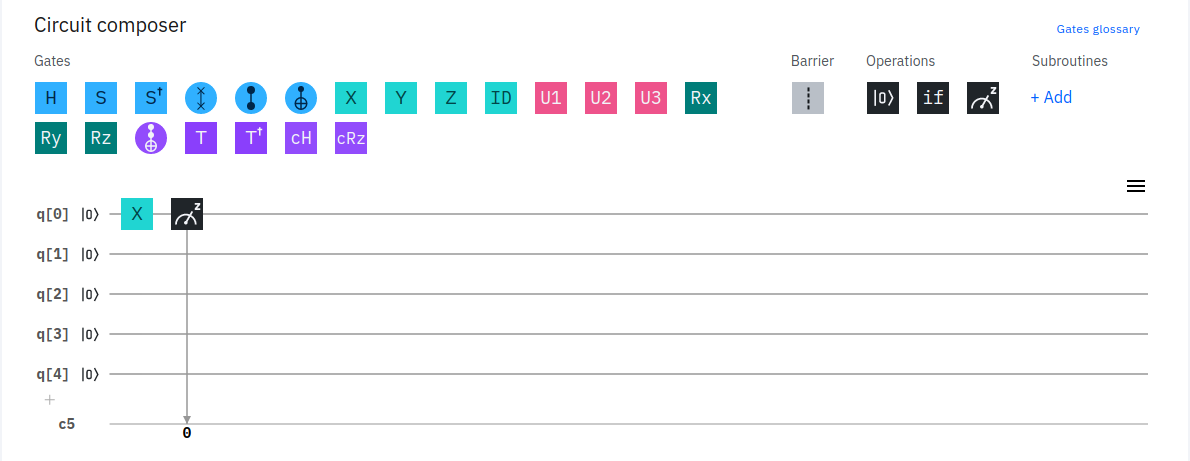
\includegraphics[width=1\textwidth]{figures/ibm_qx_composer.png} 
	\caption{Nástroj na tvorbu kvantových obvodov v IBM Quatnum Experience.}
    \label{ibm_qx_composer}
\end{figure}

Obvody je možné navrhovať aj pomocou špeciálneho jazyka OpenQASM, pomocou
editora, ktorý IBM QX obsahuje. Pri zobrazovaní výsledkov sa stav systému 
označuje pomocou klasických bitov. Teda pri navrhovaní programu pomocou
OpenQASM, je nutné definovať jednak počet kvantových a súčasne aj počet 
klasických bitov v systéme.

\begin{code}
qreg q[5];
creg c[5];
\end{code}

Je dôležité podotknúť, že kvantový bit \(\psi_0\) je v IBM QX reprezentovaný
ako \(q[0]\), \(psi_1 = q[1]\) a tak ďalej. Pri meraní sa tieto bity zobrazia
do príslušných c registrov:
\begin{itemize}
\item[] \(q[0] \rightarrow c[0]\)
\item[] \(q[1] \rightarrow c[1]\)
\item[] \(\dots\)
\end{itemize}

Po inicializácií potrebných registrov je možné pristúpiť k definovaniu 
samotného obvodu. Pre dosiahnutie obvodu ako na obrázku \ref{ibm_qx_composer}
vyvoláme aplikáciu hradla \(X\) na bite \(q[0]\) a následne využijeme meranie.

\begin{code}
x q[5];
measure q[0] -> c[0];
\end{code}

\begin{figure} 
	\centering 
	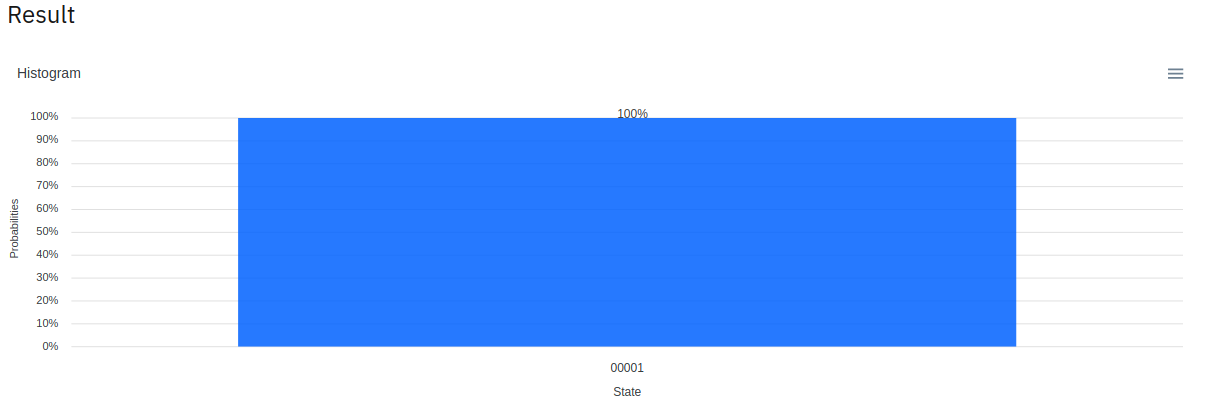
\includegraphics[width=1\textwidth]{figures/ibm_qx_results.png} 
	\caption{Výsledky experimentu z IBM Quantum Experience.}
    \label{ibm_qx_results}
\end{figure}

Výsledky experimentov sa zobrazujú v stĺpcovom diagrame, pričom stav systému
je zobrazovaný v klasických bitoch opačne ako v kvantových. Teda stav 
n-bitového systému \(\psi = \Ket{\psi_0\psi_1\psi_2 \dots \psi_{n-1}}\) je
meraný do klasického registra ako 
\[c_{n-1} \dots c_2 c_1 c_0\]
V našom prípade je
\[q[0] = X \Ket{0} =
\begin{pmatrix}
0 & 1\\
1 & 0\\
\end{pmatrix}
\binom{1}{0} = \binom{0}{1}
,\]
čo je \(1\) s pravdepodobnosťou \(1\). Výsledok na obrázku 
\ref{ibm_qx_results} zobrazuje, že kvantový systém dosiahne so \(100\%\) 
pravdepodobnosťou stav \(00001\).

\subsection{Stavy a ich zápis}

Pri výpočtoch je najviac využívaných týchto šesť stavov kvantových bitov 
\cite{Wei02}:
\begin{enumerate}
\item \(\Ket{0} = \binom{1}{0}\),
\item \(\Ket{1} = \binom{0}{1}\),
\item \(\Ket{+} = \frac{\Ket{0} + \Ket{1}}{\sqrt{2}}\),
\item \(\Ket{-} = \frac{\Ket{0} - \Ket{1}}{\sqrt{2}}\),
\item \(\Ket{\circlearrowright} = \frac{\Ket{0} - i\Ket{1}}{\sqrt{2}}\),
\item \(\Ket{\circlearrowleft} = \frac{\Ket{0} - i\Ket{1}}{\sqrt{2}}\).
\end{enumerate}
Zmena stavu kvantového bitu je možná pomocou hradiel. Existuje viacero
hradiel, ktoré možno používať v kvantových systémoch. Aplikovaním hradiel
na rôznych stavoch dosiahneme rôznu zmenu. Prehľad aplikácií základných 
hradiel je v~tabuľke \ref{hradla_vysl}.

\begin{table}
\begin{tabular}{|c|c||c|c|c|c|c|c|}
\hline
 & & \(\Ket{0}\) & \(\Ket{1}\) & \(\Ket{+}\) & \(\Ket{-}\) & \(\Ket{\circlearrowright}\) & \(\Ket{\circlearrowleft}\) \\
\hline
 & & \(\binom{1}{0}\) & \(\binom{0}{1}\) & \(\frac{1}{\sqrt{2}} \binom{1}{1}\) & \(\frac{1}{\sqrt{2}} \binom{1}{-1}\) & \(\frac{1}{\sqrt{2}}\binom{1}{i}\) & \(\frac{1}{\sqrt{2}} \binom{1}{-i}\) \\
\hline

\(X\) &  \(\begin{pmatrix}
0 & 1\\
1 & 0\\
\end{pmatrix} \) & \(\binom{0}{1}\) & \(\binom{1}{0}\) & \(\frac{1}{\sqrt{2}} \binom{1}{1}\) & \(\frac{1}{\sqrt{2}} \binom{-1}{1}\) & \(\frac{1}{\sqrt{2}} \binom{i}{1}\) & \(\frac{1}{\sqrt{2}} \binom{-i}{1}\) \\
\hline

\(Y\)  &  \(\begin{pmatrix}
0 & -i\\
i & 0\\
\end{pmatrix} \) & \(\binom{0}{i}\) & \(\binom{-i}{0}\) & \(\frac{1}{\sqrt{2}} \binom{-i}{i}\) & \(\frac{1}{\sqrt{2}} \binom{i}{i}\) & \(\frac{1}{\sqrt{2}} \binom{1}{i}\) & \(\frac{1}{\sqrt{2}} \binom{-1}{i}\) \\
\hline

\(Z\)  &  \(\begin{pmatrix}
1 & 0\\
0 & -1\\
\end{pmatrix} \) & \(\binom{1}{0}\) & \(\binom{0}{-1}\) & \(\frac{1}{\sqrt{2}} \binom{1}{-1}\) & \(\frac{1}{\sqrt{2}} \binom{1}{1}\) & \(\frac{1}{\sqrt{2}} \binom{1}{-i}\) & \(\frac{1}{\sqrt{2}} \binom{1}{i}\) \\
\hline

\(H\)  &  \(\frac{1}{\sqrt{2}}\begin{pmatrix}
1 & 1\\
1 & -1\\
\end{pmatrix} \) & \(\frac{1}{\sqrt{2}}\binom{1}{1}\) & \(\frac{1}{\sqrt{2}}\binom{1}{-1}\) & \(\binom{1}{0}\) & \(\binom{0}{1}\) & \(\frac{1}{\sqrt{2}} \binom{\frac{1+i}{\sqrt{2}}}{\frac{1-i}{\sqrt{2}}}\) & \(\frac{1}{\sqrt{2}} \binom{\frac{1-i}{\sqrt{2}}}{\frac{1+i}{\sqrt{2}}}\) \\
\hline

\(S\)  &  \(\begin{pmatrix}
1 & 0\\
0 & i\\
\end{pmatrix} \) & \(\binom{1}{0}\) & \(\binom{0}{i}\) & \(\frac{1}{\sqrt{2}} \binom{1}{i}\) & \(\frac{1}{\sqrt{2}} \binom{1}{-i}\) & \(\frac{1}{\sqrt{2}} \binom{1}{-1}\) & \(\frac{1}{\sqrt{2}} \binom{1}{1}\) \\
\hline

\(S^{\dag}\)  &  \(\begin{pmatrix}
1 & 0\\
0 & -i\\
\end{pmatrix} \) & \(\binom{1}{0}\) & \(\binom{0}{-i}\) & \(\frac{1}{\sqrt{2}} \binom{1}{-i}\) & \(\frac{1}{\sqrt{2}} \binom{1}{i}\) & \(\frac{1}{\sqrt{2}} \binom{1}{1}\) & \(\frac{1}{\sqrt{2}} \binom{1}{-1}\) \\
\hline

\(T\)  &  \(\begin{pmatrix}
1 & 0\\
0 & \frac{1+i}{\sqrt{2}}\\
\end{pmatrix} \) & \(\binom{1}{0}\) & \(\binom{0}{\frac{1+i}{\sqrt{2}}}\) & \(\frac{1}{\sqrt{2}} \binom{1}{\frac{1+i}{\sqrt{2}}}\) & \(\frac{1}{\sqrt{2}} \binom{1}{\frac{-1-i}{\sqrt{2}}}\) & \(\frac{1}{\sqrt{2}} \binom{1}{\frac{-1+i}{\sqrt{2}}}\) & \(\frac{1}{\sqrt{2}} \binom{1}{\frac{1-i}{\sqrt{2}}}\) \\
\hline

\(T^{\dag}\)  &  \(\begin{pmatrix}
1 & 0\\
0 & \frac{1-i}{\sqrt{2}}\\
\end{pmatrix} \) & \(\binom{1}{0}\) & \(\binom{0}{\frac{1-i}{\sqrt{2}}}\) & \(\frac{1}{\sqrt{2}} \binom{1}{\frac{1-i}{\sqrt{2}}}\) & \(\frac{1}{\sqrt{2}} \binom{1}{\frac{-1+i}{\sqrt{2}}}\) & \(\frac{1}{\sqrt{2}} \binom{1}{\frac{1+i}{\sqrt{2}}}\) & \(\frac{1}{\sqrt{2}} \binom{1}{\frac{-1-i}{\sqrt{2}}}\) \\
\hline
\end{tabular}

\caption{\label{hradla_vysl} Tabuľka stavov kvantových bitov a výsledky 
aplikácií hradiel na tieto stavy.}
\end{table}

\subsection{Operácie kvantových hradiel}
\label{op_kvan_hradiel}
Existuje veľké množstvo hradiel. No v našom pravdepodobnostnom modely budeme
využívať osem základných hradiel, ktoré sú najviac využívané. V tejto časti
ukážeme ako hradlá \(X, Y, Z, H, S, S^{\dag}, T\) a \(T^{\dag}\) menia stav
kvantového bitu \cite{Nie+00}. Definujme bit \(\ket{\psi} = \binom{\alpha}{\beta}\), na 
ktorom aktivujeme dané hradlá.
\[X\ket{\psi} = 
\begin{pmatrix}
0 & 1 \\
1 & 0 \\
\end{pmatrix}\binom{\alpha}{\beta} = \binom{\beta}{\alpha} = \beta\ket{0} + \alpha\ket{1}\]

\[Y\ket{\psi} = 
\begin{pmatrix}
0 & -i \\
i & 0 \\
\end{pmatrix}\binom{\alpha}{\beta} = \binom{-i\beta}{i\alpha} = -i\beta\ket{0} + i\alpha\ket{1}\]

\[Z\ket{\psi} = 
\begin{pmatrix}
1 & 0 \\
0 & -1 \\
\end{pmatrix}\binom{\alpha}{\beta} = \binom{\alpha}{-\beta} = \alpha\ket{0} - \beta\ket{1}\]

\[H\ket{\psi} = \frac{1}{\sqrt{2}}
\begin{pmatrix}
1 & 1 \\
1 & -1 \\
\end{pmatrix}\binom{\alpha}{\beta} = \frac{1}{\sqrt{2}}\binom{\alpha + \beta}{\alpha - \beta} = \frac{\alpha + \beta}{\sqrt{2}}\ket{0} + \frac{\alpha - \beta}{\sqrt{2}}\ket{1}\]

\[S\ket{\psi} = 
\begin{pmatrix}
1 & 0 \\
0 & i \\
\end{pmatrix}\binom{\alpha}{\beta} = \binom{\alpha}{i\beta} = \alpha\ket{0} + i\beta\ket{1}\]

\[S^{\dag}\ket{\psi} = 
\begin{pmatrix}
1 & 0 \\
0 & -i \\
\end{pmatrix}\binom{\alpha}{\beta} = \binom{\alpha}{-i\beta} = \alpha\ket{0} - i\beta\ket{1}\]

\[T\ket{\psi} = 
\begin{pmatrix}
1 & 0 \\
0 & \frac{1 + i}{\sqrt{2}} \\
\end{pmatrix}\binom{\alpha}{\beta} = \binom{\alpha}{\frac{1 + i}{\sqrt{2}}\beta} = \alpha\ket{0} + \frac{1 + i}{\sqrt{2}}\beta\ket{1}\]

\[T^{\dag}\ket{\psi} = 
\begin{pmatrix}
1 & 0 \\
0 & \frac{1 - i}{\sqrt{2}} \\
\end{pmatrix}\binom{\alpha}{\beta} = \binom{\alpha}{\frac{1 - i}{\sqrt{2}}\beta} = \alpha\ket{0} + \frac{1 - i}{\sqrt{2}}\beta\ket{1}\]

% !TEX root = ../thesis.tex

\chapter{Pravdepodobnostná analýza kvantových obvodov}
\label{pravAnalL}

V predošlých kapitolách bola vysvetlená problematika kvantových obvodov.
Našou úlohou je merať stavy kvantových bitov v rôznych časových okamihoch.
Je možné zostrojiť nekonečné množstvo rôznych kvantových obvodov,
a preto v tejto časti priblížime spôsob tohto merania.
Vo všeobecnosti môžme rozdeliť kvantové obvody na dva druhy, v ktorých 
meranie má iný charakter. Sú to obvody s nepreviazanými bitmi a obvody s 
previazanými kvantovými bitmi. Totižto pri nepreviazaných bitoch,
ako už vychádza z názvu, nedochádza k ovplyvňovaniu stavu bitu inými 
kvantovými bitmi. A naopak ak sú jednotlivé bity previazané, ich stav silno
závisí od stavu ostatných bitov.

\section{Analýza nepreviazaných stavov}

\begin{figure} 
	\centering 
	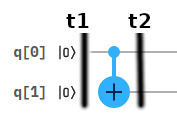
\includegraphics[width=.4\textwidth]{figures/simpleCircuit2.png} 
	\caption{Jednoduchý kvantový obvod (namodelovaný v IBM Quantum Experience)}
    \label{obvod}
\end{figure}

Na obrázku \ref{obvod} je vygenerovaný jednoduchý kvantový obvod pomocou
nástroja IBM Quantum Experience. V jazyku OpenQASM je možné definovať tento
obvod ako:
\begin{code}
qreg q[2];
creg c[2];

cx q[0],q[1];
\end{code}

V tomto obvode sú dva kvantové bity, ktoré prechádzajú 
hradlom CNOT. Pre zachovanie notácie budeme ďalej označovať tieto bity ako 
\(\psi_0\) a \(\psi_1\). Označili sme dva časové úseky \(t_1\) a \(t_2\).
\(t_1\) označuje čas na začiatku programu a \(t_2\) je časový okamih, v ktorom
prebehla aktivácia hradla CNOT.
 Z kvantového obvodu je zrejmé, že v čase \(t_1\) 
sú oba kvantové bity v stave
\(\ket{0}\). Tento fakt ale nie je pre nás zaujímavý. Pozrieme sa na meranie 
pravdepodobnosti dosiahnutia  
namerania stavov \(\ket{00}, \ket{01}, \ket{10}\) a \(\ket{11}\).

Vieme, že platí \(\ket{\psi_0} = \binom{\alpha_0}{\beta_0}\) a  
\(\ket{\psi_1} = \binom{\alpha_1}{\beta_1}\), a teda pre celkový stav \(\psi\) 
platí 
\[
\ket{\psi} = \ket{\psi_0} \otimes \ket{\psi_1} = \binom{\alpha_0}{\beta_0}
\otimes \binom{\alpha_1}{\beta_1} = 
\begin{pmatrix}
    \alpha_0\alpha_1 \\
    \alpha_0\beta_1 \\
    \beta_0\alpha_1 \\
    \beta_0\beta_1
\end{pmatrix}
\]
Z toho vyplýva, že celkový stav \(\ket{\psi}\) v čase \(t_1\) nadobúda 
hodnoty
\begin{itemize}
    \item[] \(\ket{00}\) s pravdepodobnosťou \(\Vert \alpha_0\alpha_1 \Vert^2\)
    \item[] \(\ket{01}\) s pravdepodobnosťou \(\Vert \alpha_0\beta_1 \Vert^2\)
    \item[] \(\ket{10}\) s pravdepodobnosťou \(\Vert \beta_0\alpha_1 \Vert^2\)
    \item[] \(\ket{11}\) s pravdepodobnosťou \(\Vert \beta_0\beta_1 \Vert^2\)
\end{itemize}

Toto tvrdenie platí, pretože platí 
\(\ket{\psi_0} = \alpha_0\ket{0} + \beta_0\ket{1}\), čiže 
\(|\alpha_0|^2 + |\beta_0|^2 = 1\), z čoho vyplýva, že 
\begin{itemize}
    \item[] \(\ket{\psi_0}\) nadobúda hodnotu 0 s 
pravdepodobnosťou \(|\alpha_0|^2\) a 
    \item[] \(\ket{\psi_0}\) nadobúda hodnotu 1 s 
pravdepodobnosťou \(|\beta_0|^2\).
\end{itemize}
Obdobne to platí aj pre \(\ket{\psi_1}\). K rovnakému záveru sa dopracujeme
aj pomocou 
\[\ket{\psi} = \ket{\psi_0} \otimes \ket{\psi_1} = 
(\alpha_0\ket{0} + \beta_0\ket{1}) \otimes  (\alpha_1\ket{0} + \beta_1\ket{1}) =
\]
\[
\alpha_0\alpha_1 (\ket{0} \otimes \ket{0}) +  
\alpha_0\beta_1 (\ket{0} \otimes \ket{1}) + 
\beta_0\alpha_1 (\ket{1} \otimes \ket{0}) + 
\beta_0\beta_1 (\ket{1} \otimes \ket{1}), 
\]
čo by sme mohli vyjadriť aj iným zápisom ako 
\(
\alpha_{00}\ket{00} + \alpha_{01}\ket{01} + 
\alpha_{10}\ket{10} + \alpha_{11}\ket{11}
\), pričom súčet noriem musí byť rovný 1.
\[
|\alpha_{00}|^2 + |\alpha_{01}|^2 + |\alpha_{10}|^2 + |\alpha_{11}|^2 = 1\]

\section{Analýza previazaných stavov}

Pri meraní stavov v čase \(t_2\), už nemožno dostať výsledný stav \(\psi\)
priamym využitím tenzorového súčinu. Pri prechode hradom CNOT môžu nastať
dve situácie:
\begin{enumerate}
    \item Kvantový bit \(\psi_0\), ktorý je kontrólnym bitom, je v stave 
\(\ket{1}\) a teda nastane preklopenie bitu \(\psi_1\), čo je cieľovým bitom,
pomocou hradla X,
    \item Kvantový bit \(\psi_0\) nie je v stave \(\ket{1}\) a teda bit 
\(\psi_1\) pokračuje bez zmeny.
\end{enumerate}

Z toho je jasné, že v každom prípade sa stav \(\ket{\psi_0}\) nemení no
stav \(\ket{\psi_1}\) nadobúda hodnotu:
\begin{itemize}
    \item \(\ket{\psi_1}\) s pravdepodobnosťou \(|\alpha_0|^2\),
    \item \(X\ket{\psi_1}\) s pravdepodobnosťou \(|\beta_0|^2\).
\end{itemize}

A teda s pravdepodobnosťou \(|\alpha_0|^2\) systém skončí v stave
\[\Ket{\psi} =  \Ket{\psi_0} \otimes \Ket{\psi_1} = 
(\alpha_0\ket{0} + \beta_0\ket{1}) \otimes  (\alpha_1\ket{0} + \beta_1\ket{1})
\]
a s pravdepodobnosťou \(|\beta_0|^2\) dosiahne stav
\[\Ket{\psi} =  \Ket{\psi_0} \otimes X\Ket{\psi_1} = 
(\alpha_0\ket{0} + \beta_0\ket{1}) \otimes  (\beta_1\ket{0} + \alpha_1\ket{1})
\]

Po zarátaní oboch možností dostávame, že celkový stav \(\ket{\psi}\) v čase 
\(t_2\) nadobúda hodnoty 
\begin{itemize}
    \item[] \(\ket{00}\) s pravdepodobnosťou \((|\alpha_0\alpha_1|^2 \times |\alpha_0|^2) + (|\alpha_0\beta_1|^2 \times |\beta_0|^2)\)
    \item[] \(\ket{01}\) s pravdepodobnosťou \((|\alpha_0\beta_1|^2 \times |\alpha_0|^2) + (|\alpha_0\alpha_1|^2 \times |\beta_0|^2)\)
    \item[] \(\ket{10}\) s pravdepodobnosťou \((|\beta_0\alpha_1|^2 \times |\alpha_0|^2) + (|\beta_0\beta_1|^2 \times |\beta_0|^2)\)
    \item[] \(\ket{11}\) s pravdepodobnosťou \((|\beta_0\beta_1|^2 \times |\alpha_0|^2) + (|\beta_0\alpha_1|^2 \times |\beta_0|^2)\)
\end{itemize}


Berme v úvahu to, že v príklade sme využili hradlo \(CNOT\). Je samozrejmé, že
v obvode môže dôjsť k previazaniu viacerých bitov na rôznych miestach.
Takisto je možné vo viacbitovom systéme využiť haradlo \(CCNOT\) resp. 
\(C^{n}NOT\), kde máme viacero kontrólnych bitov a cieľový bit sa preklápa
za predpokladu, že všetky kontrólne bity majú stav \(\ket{1}\).
Zisťujeme, že odvodzovanie je netriviálne a tento problém je nutné riešiť
pomocou pravdepodobnostného rozhodovacieho stromu (o tom v ďalších kapitolách).

% !TEX root = ../thesis.tex

\chapter{Meranie kvantových obvodov}

Jediným spôsobom ako zistiť skutočný stav kvnatového obvodu je meraním.
Merať možno všetky bity súčasne ako aj jednotlivé kvantové bity samostatne.

\section{Princíp merania kvantových obvodov}

Kvantový bit môže existovať v nekonečnom množstve stavov. Meranie si môžme 
predstaviť ako prevod stavov kvantových bitov do stavu klasického digitálneho
systému \cite{Nie10}. Pre príklad môžeme reprezentovať kvantový stav 
\(\alpha\ket{0} + \beta\ket{1}\) pomocou nulového a excitovaného stavu atómu.
Skutočný kvantový počítač by tak mohol merať tieto stavy. Pri meraní by 
daný atóm skolaboval do jedného zo stavov \(\ket{0}\) alebo \(\ket{1}\).
Pre kolabovanie samozrejme rovnako platí to, že do jednotlivých stavov by
sa atóm dostal s pravdepodobnosťami \(|\alpha|^2\) respektíve \(|\beta|^2\).


Pri každom fyzikálnom meraní nastáva určitá nepresnosť merania. Takisto 
pri meraní môže dokonca nastať zničenie obvodu. To vyplíva z toho, že pri
skolabovanom kvantovom bite nastáva zmena fizykálnych vlastností daného bitu. 

\section{Fiktívne meranie}

Našim cieľom je navrhnúť pravdepodobnostný model, ktorý by umožnil merať
stavy kvantových obvodov aj bez kolabovania jednotlivých kvantových bitov.

\subsection{Experiment 1}
Navrhnime kvantový obvod s dvoma bitmi. Označme ich \(\ket{\psi_0}\) a 
\(\ket{\psi_1}\). V prvom kroku aplikujeme Hadamardovo hrado na bit 
\(\ket{\psi_0}\). Nasledovať budú dve \(CNOT\) hradlá, s opačnými kontrólnymi 
a cieľovými bitmi. V IBM QX je tento obvod reprezenovaný ako 
\begin{code}
qreg q[2];
creg c[2];

h q[0];
cx q[0],q[1];
cx q[1],q[0];
\end{code}
Jeho grafické zobrazenie je na obrázku \ref{expr1_circuit}, aj s označenými
časovými úsekmi, v ktorých bude meraný stav systému. 

\begin{figure} 
	\centering 
	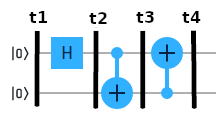
\includegraphics[width=.6\textwidth]{figures/expr1_circuit.png} 
	\caption{Obvod experimentu 1 s označenými časovými úsekmi meraní.}
    \label{expr1_circuit}
\end{figure}

\subsection*{Teoretická analýza}
Kvantové bity \(\ket{\psi_0}\) a \(\ket{\psi_2}\) sú definované ako 
\[\ket{\psi_0} = \alpha_0\ket{0} + \beta_0\ket{1}\]
\[\ket{\psi_1} = \alpha_1\ket{0} + \beta_1\ket{1}\]
, a teda je zrejmé, že v čase \(t_1\) pre celkový stav \(\ket{\psi}\) platí 
\[\ket{\psi} = \ket{\psi_0} \otimes \ket{\psi_1} = \alpha_0\alpha_1\ket{00} + \alpha_0\beta_1\ket{01} + \beta_0\alpha_1\ket{10} + \beta_0\beta_1\ket{11}\]

Z čoho jasne vyplíva, že systém nadobudne stav
    \begin{itemize}
        \item[] \(\ket{00}\) s pravdepodobnosťou \(|\alpha_0\alpha_1 |^2\)
        \item[] \(\ket{01}\) s pravdepodobnosťou \(| \alpha_0\beta_1 |^2\)
        \item[] \(\ket{10}\) s pravdepodobnosťou \(| \beta_0\alpha_1 |^2\)
        \item[] \(\ket{11}\) s pravdepodobnosťou \(| \beta_0\beta_1 |^2\) 
    \end{itemize}

Po prechode Hadamardovim hradlom, v čase \(t_2\) kvantové bity zmenia svoj stav
 na
\[\ket{\psi_0} = \frac{\alpha_0 + \beta_0}{\sqrt{2}}\ket{0} + \frac{\alpha_0 - \beta_0}{\sqrt{2}}\ket{1}\]
\[\ket{\psi_1} = \alpha_1\ket{0} + \beta_1\ket{1}\]

, a teda pre celkový stav \(\ket{\psi}\) bude platiť
\[\ket{\psi} = \frac{\alpha_0 + \beta_0}{\sqrt{2}}\alpha_1\ket{00} + \frac{\alpha_0 + \beta_0}{\sqrt{2}}\beta_1\ket{01} + \frac{\alpha_0 - \beta_0}{\sqrt{2}}\alpha_1\ket{10} + \frac{\alpha_0 - \beta_0}{\sqrt{2}}\beta_1\ket{11}\]

Kvantoý systém kolabuje v čase \(t_2\) do stavu
    \begin{itemize}
        \item[] \(\ket{00}\) s pravdepodobnosťou \(|\frac{\alpha_0 + \beta_0}{\sqrt{2}}\alpha_1|^2\)
        \item[] \(\ket{01}\) s pravdepodobnosťou \(|\frac{\alpha_0 + \beta_0}{\sqrt{2}}\beta_1|^2\)
        \item[] \(\ket{10}\) s pravdepodobnosťou \(|\frac{\alpha_0 - \beta_0}{\sqrt{2}}\alpha_1|^2\)
        \item[] \(\ket{11}\) s pravdepodobnosťou \(|\frac{\alpha_0 - \beta_0}{\sqrt{2}}\beta_1|^2\) 
    \end{itemize}

Zmena nastáva v čase \(t_3\), po prechode \(CNOT\) hradlom. Bit \(\ket{\psi_1}\)
bude preklopený len v prípade, že \(\ket{\psi_0}\) kolabuje do stavu 
\(\ket{1}\). A teda nastávajú dve možnosti. S pravdepodobnosťou 
\(|\frac{\alpha_0 + \beta_0}{\sqrt{2}}|^2\), ktorú označíme ako \(P^{t3}_1\) sa 
stavy kvantových bitov nezmenia
\[\ket{\psi_0} = \frac{\alpha_0 + \beta_0}{\sqrt{2}}\ket{0} + \frac{\alpha_0 - \beta_0}{\sqrt{2}}\ket{1}\]
\[\ket{\psi_1} = \alpha_1\ket{0} + \beta_1\ket{1}\]

Naopak, bit \(\ket{\psi_0}\) kolabuje do stavu \(\ket{1}\) s pravdepodobnosťou
\(|\frac{\alpha_0 - \beta_0}{\sqrt{2}}|^2\) (označme \(P^{t3}_{2}\)), a teda 
v tomto prípade nastáva zmena v kvantovom bite \(\ket{\psi_1}\)
\[\ket{\psi_1} = \beta_1\ket{0} + \alpha_1\ket{1}\]

Platí, že systém v čase \(t_3\) môže kolabovať do stavu
    \begin{itemize}
        \item[] \(\ket{00}\) s pravdepodobnosťou \((|\frac{\alpha_0 + \beta_0}{\sqrt{2}}\alpha_1|^2 \times P^{t3}_1) + (|\frac{\alpha_0 + \beta_0}{\sqrt{2}}\beta_1|^2 \times P^{t3}_{2})\)
        \item[] \(\ket{01}\) s pravdepodobnosťou \((|\frac{\alpha_0 + \beta_0}{\sqrt{2}}\beta_1|^2 \times P^{t3}_1 ) +(|\frac{\alpha_0 + \beta_0}{\sqrt{2}}\alpha_1|^2 \times P^{t3}_2)\)
        \item[] \(\ket{10}\) s pravdepodobnosťou \((|\frac{\alpha_0 - \beta_0}{\sqrt{2}}\alpha_1|^2 \times P^{t3}_1) +  (|\frac{\alpha_0 - \beta_0}{\sqrt{2}}\beta_1|^2 \times P^{t3}_2)\)
        \item[] \(\ket{11}\) s pravdepodobnosťou \((|\frac{\alpha_0 - \beta_0}{\sqrt{2}}\beta_1|^2 \times P^{t3}_1) +(|\frac{\alpha_0 - \beta_0}{\sqrt{2}}\alpha_1|^2 \times P^{t3}_2)\) 
    \end{itemize}


Poslendé meranie v tomto experimente je označené ako \(t_4\). Opäť nástáva
aktivácia \(CNOT\) hradla a teda podmienená zmena stavov kvantových bitov.
V každom prípade bit \(\ket{\psi_1}\) ostane nezmenený. No už teraz vychádzame 
z dvoch možností. Teda môžu nastať celkovo štyri pípady. V tabuľke 
\ref{expr1_t4_states} sú všetky možné zmeny stavov \(\ket{\psi_0}\) a
\(\ket{\psi_1}\).

\begin{table}
\centering
\begin{tabular}{|l|c|}
\hline
\textbf{Pravdepodobnosť} & \textbf{Stavy \(\ket{\psi_0}\) a \(\ket{\psi_1}\)} \\
\hline
\(P^{t4}_1 = |\frac{\alpha_0 + \beta_0}{\sqrt{2}}\alpha_1|^2\) & 
\(\ket{\psi_0} = \frac{\alpha_0 + \beta_0}{\sqrt{2}}\ket{0} + \frac{\alpha_0 - \beta_0}{\sqrt{2}}\ket{1}\) \\
& \(\ket{\psi_1} = \alpha_1\ket{0} + \beta_1\ket{1}\) \\
\hline

\(P^{t4}_2 = |\frac{\alpha_0 + \beta_0}{\sqrt{2}}\beta_1|^2\) & 
\(\ket{\psi_0} = \frac{\alpha_0 - \beta_0}{\sqrt{2}}\ket{0} + \frac{\alpha_0 + \beta_0}{\sqrt{2}}\ket{1}\) \\
& \(\ket{\psi_1} = \alpha_1\ket{0} + \beta_1\ket{1}\) \\
\hline

\(P^{t4}_3 = |\frac{\alpha_0 - \beta_0}{\sqrt{2}}\beta_1|^2\) & 
\(\ket{\psi_0} = \frac{\alpha_0 + \beta_0}{\sqrt{2}}\ket{0} + \frac{\alpha_0 - \beta_0}{\sqrt{2}}\ket{1}\) \\
& \(\ket{\psi_1} = \beta_1\ket{0} + \alpha_1\ket{1}\) \\
\hline

\(P^{t4}_4 = |\frac{\alpha_0 - \beta_0}{\sqrt{2}}\alpha_1|^2\) & 
\(\ket{\psi_0} = \frac{\alpha_0 - \beta_0}{\sqrt{2}}\ket{0} + \frac{\alpha_0 + \beta_0}{\sqrt{2}}\ket{1}\) \\
& \(\ket{\psi_1} = \beta_1\ket{0} + \alpha_1\ket{1}\) \\
\hline

\end{tabular}

\caption{\label{expr1_t4_states} Tabuľka stavov kvantových bitov a pravedpodobností
nastatia týchto stavov v čase \(t_4\) experimentu 1.}
\end{table}

Čiže celkový stav \(\ket{\psi}\) nadobudne stav
    \begin{itemize}
        \item[] \(\ket{00}\) s pravdepodobnosťou \\
\((|\frac{\alpha_0 + \beta_0}{\sqrt{2}}\alpha_1|^2 \times P^{t4}_1) + (|\frac{\alpha_0 - \beta_0}{\sqrt{2}}\alpha_1|^2 \times P^{t4}_2) + (|\frac{\alpha_0 + \beta_0}{\sqrt{2}}\beta_1|^2 \times P^{t4}_3) + (|\frac{\alpha_0 - \beta_0}{\sqrt{2}}\beta_1|^2 \times P^{t4}_4)\)

        \item[] \(\ket{01}\) s pravdepodobnosťou \\
 \((|\frac{\alpha_0 + \beta_0}{\sqrt{2}}\beta_1|^2 \times P^{t4}_1) + (|\frac{\alpha_0 - \beta_0}{\sqrt{2}}\beta_1|^2 \times P^{t4}_2) + (|\frac{\alpha_0 + \beta_0}{\sqrt{2}}\alpha_1|^2 \times P^{t4}_3) + (|\frac{\alpha_0 - \beta_0}{\sqrt{2}}\alpha_1|^2 \times P^{t4}_4)\)

        \item[] \(\ket{10}\) s pravdepodobnosťou \\ 
\((|\frac{\alpha_0 - \beta_0}{\sqrt{2}}\alpha_1|^2 \times P^{t4}_1) + (|\frac{\alpha_0 + \beta_0}{\sqrt{2}}\alpha_1|^2 \times P^{t4}_2) + (|\frac{\alpha_0 - \beta_0}{\sqrt{2}}\beta_1|^2 \times P^{t4}_3) + (|\frac{\alpha_0 + \beta_0}{\sqrt{2}}\beta_1|^2 \times P^{t4}_4)\)

        \item[] \(\ket{11}\) s pravdepodobnosťou \\
\((|\frac{\alpha_0 - \beta_0}{\sqrt{2}}\beta_1|^2 \times P^{t4}_1) + (|\frac{\alpha_0 + \beta_0}{\sqrt{2}}\beta_1|^2 \times P^{t4}_2) + (|\frac{\alpha_0 - \beta_0}{\sqrt{2}}\alpha_1|^2 \times P^{t4}_3) + (|\frac{\alpha_0 + \beta_0}{\sqrt{2}}\alpha_1|^2 \times P^{t4}_4)\)
    \end{itemize}

\subsection*{Výpočet pravdepodobností pomocou pravdepodobnostného modelu}
Pre použitie pravdepodobnostného modelu je nutné definovať obvod v jazyku 
Haskell. Vyjadrime jednotlivé hradlá a rozdeľme ich po vertikálnych leveloch.
\begin{code}
let l1 = Level [E, E] True
    l2 = Level [H, E] True
    l3 = Level [Cc, Ct] True
    l4 = Level [Ct, Cc] True
\end{code}
Pre meranie aj v čase \(t_1\), čiže ešte pred aktiváciou akéhokoľvek hradla,  
sme vložili jeden prázdny level navyše. Uložme tento obvod do spoločného listu
a definujme aj stromové štruktúry pre stavy a výsledky.
\begin{code}
c = [l1, l2, l3, l4]
st = StateTree 1 [q0, q0] []
rt = RT st []
\end{code}

Teraz už len spustime pravdepodobnostný model a uložme výsledky.
\begin{code}
let resultRT = processCircuit c rt
\end{code}

\begin{table}
\centering
\begin{tabular}{|c|}
\hline
1.0 \\ 
00 \\ 
\hline
\end{tabular}

\begin{tabular}{|c|c|}
\hline
0.5000000000000001 & 0.4999999999999999 \\ 
00 & 10 \\ 
\hline
\end{tabular}

\begin{tabular}{|c|c|c|c|}
\hline
0.25 & 0.2499999999999999 & 0.2500000000000001 & 0.25 \\ 
01 & 11 & 00 & 10 \\ 
\hline
\end{tabular}

\begin{tabular}{|c|c|c|c|c|c|}
\hline
0.25 & 0.2499999999999999 & 0.0 & 0.0 & 0.2500000000000001 & 0.25 \\ 
01 & 11 & 01 & 11 & 00 & 10 \\ 
\hline
\end{tabular}
\caption{\label{expr1_vystup} Výstup pravdepodobnostného modelu pre experiment 1
. Ohraničené riadky vymedzujú výsledky v jednotlivých časoch merania. Každá
bunka obsahuje pravdepodobnosť dosiahnutia stavu a daný stav systému.}
\end{table}

Pre vstupy kde na začiatku obvodu je \(\ket{\psi_0} = \ket{0}\) a zároveň
\(\ket{\psi_1} = \ket{0}\) nám model vypočítal výsledky, ktoré sú zaznamenané
v tabuľke \ref{expr1_vystup}. Každý ohraničený riadok predstavuje časový úsek.
Každá bunka potom obsahuje možný stav systému v daný časový úsek, kde horné
číslo je pravdepodobnosť dosiahnutia tohto stavu v rozmedzí \(0\) až \(1\) a 
spodná hodnota určuje daný stav v tvare \(\psi_0\psi_1\).

\begin{figure} 
	\centering 
	\includegraphics[width=.8\textwidth]{figures/expr1_qx_results.png} 
	\caption{Výsledky experimentu 1 z Quantum Experience so zvýraznenými 
údajmi.}

    \label{expr1_qx_results}
\end{figure}

Porovnajme naše výsledky so symulátorom IBM Quantum Experience. V IBM QX
bolo nutné vykonať štyri experimenty s rôznim časom merania, nakoľko tento
symulátor nepodporuje fiktívne meranie. Dosiahnuté výsledky sú na obrázku
\ref{expr1_qx_results}. Pripomeňme, že notácia dosiahnutých stavov v IBM QX
je \(\psi_1\psi_0\), teda v opačnom poradí ako zápis v našej tabuľke. V 
prvích dvoch merania sú výsledky totožné. Rozdiel nastáva pri prechode hradlom
\(CNOT\). Pravdepodobnostný model, ktorý využívame, funguje na istom 
matematickom aparáte. IBM QX je ale symulátor kantového počítača a teda môže 
brať do úvahy iné fyzikálne vlastnosti kvatových bitov, ktoré môžu vysvetľovať
rozdiel v našich výsledkoch.

\subsection{Experiment 2}
\begin{figure} 
	\centering 
	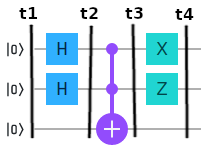
\includegraphics[width=.5\textwidth]{figures/expr2_circuit.png} 
	\caption{Obvod experimentu 2 s označenými časovými úsekmi meraní.}

    \label{expr2_circuit}
\end{figure}

Definujme kvantový obvod tak ako je na obrázku \ref{expr2_circuit}. Majme 
tri kvantové bity, ktoré označíme ako \(\psi_0\), \(\psi_1\) a \(\psi_2\).
Na prvých dvoch bitoch aktivujeme Hadamardové hradlá a potom tieto bity 
využijeme ako kontrólne bity v Tuffliho hradle. Nakoniec aplikujeme hradlo 
\(X\) a \(Z\).

V OpenQASM je tento obvod zostrojený ako
\begin{code}
qreg q[3];
creg c[3];

h q[0];
h q[1];
ccx q[0],q[1],q[2];
x q[0];
z q[1];
\end{code}

\subsection*{Teoretická analýza}
Stále platí, že
\[\ket{\psi_0} = \alpha_0\ket{0} + \beta_0\ket{1}\]
\[\ket{\psi_1} = \alpha_1\ket{0} + \beta_1\ket{1}\]
\[\ket{\psi_2} = \alpha_2\ket{0} + \beta_2\ket{1}\]
Zistiť stav systému v čase \(t_1\) je preto priamočiare
\[\ket{\psi} = \ket{\psi_0} \otimes \ket{\psi_1} \otimes \ket{\psi_2}\]

V čase \(t_2\) nastala aktivácia hradla \(H\) a preto sa zmení stav kvantových
bitov na 
\[\ket{\psi_0} = \frac{\alpha_0 + \beta_0}{\sqrt{2}}\ket{0} + \frac{\alpha_0 - \beta_0}{\sqrt{2}}\ket{1}\]
\[\ket{\psi_1} = \frac{\alpha_1 + \beta_1}{\sqrt{2}}\ket{0} + \frac{\alpha_1 - \beta_1}{\sqrt{2}}\ket{1}\]
\[\ket{\psi_2} = \alpha_2\ket{0} + \beta_2\ket{1}\]
Vyjadrenie pravdepodobností dosiahnutia stavov z meraní \(1\) a \(2\) sú 
zaznamenané v tabuľke \ref{expr2_tanal12}

\begin{table}
\centering
\begin{tabular}{|c|c|c|}
\hline
\textbf{Stav} & \multicolumn{2}{c|}{\textbf{Pravdepodobnosti}} \\
 & \(t_1\) & \(t_2\) \\
\hline
\(\ket{000}\) & \(|\alpha_0\alpha_1\alpha_2|^2\) & 
\(|\frac{\alpha_0 + \beta_0}{\sqrt{2}} \frac{\alpha_1 + \beta_1}{\sqrt{2}} \alpha_2|^2\) \\

\(\ket{001}\) & \(|\alpha_0\alpha_1\beta_2|^2\) & 
\(|\frac{\alpha_0 + \beta_0}{\sqrt{2}} \frac{\alpha_1 + \beta_1}{\sqrt{2}} \beta_2|^2\)  \\
%\hline

\(\ket{010}\) & \(|\alpha_0\beta_1\alpha_2|^2\) & 
\(|\frac{\alpha_0 + \beta_0}{\sqrt{2}} \frac{\alpha_1 - \beta_1}{\sqrt{2}} \alpha_2|^2\)   \\
%\hline

\(\ket{011}\) & \(|\alpha_0\beta_1\beta_2|^2\) &
\(|\frac{\alpha_0 + \beta_0}{\sqrt{2}} \frac{\alpha_1 - \beta_1}{\sqrt{2}} \beta_2|^2\)  \\
%\hline

\(\ket{100}\) & \(|\beta_0\alpha_1\alpha_2|^2\) &
\(|\frac{\alpha_0 - \beta_0}{\sqrt{2}} \frac{\alpha_1 + \beta_1}{\sqrt{2}} \alpha_2|^2\)   \\
%\hline

\(\ket{101}\) & \(|\beta_0\alpha_1\beta_2|^2\) &
\(|\frac{\alpha_0 - \beta_0}{\sqrt{2}} \frac{\alpha_1 + \beta_1}{\sqrt{2}} \beta_2|^2\)   \\
%\hline

\(\ket{110}\) & \(|\beta_0\beta_1\alpha_2|^2\) & 
 \(|\frac{\alpha_0 - \beta_0}{\sqrt{2}} \frac{\alpha_1 - \beta_1}{\sqrt{2}} \alpha_2|^2\)  \\
%\hline

\(\ket{111}\) & \(|\beta_0\beta_1\beta_2|^2\) & 
\(|\frac{\alpha_0 - \beta_0}{\sqrt{2}} \frac{\alpha_1 - \beta_1}{\sqrt{2}} \beta_2|^2\)   \\
\hline

\end{tabular}

\caption{\label{expr2_tanal12} Vyjadrenie meraní pravdepodobnosti v čase 
\(t_1\) a \(t_2\) experimentu 2.}
\end{table}


Časový okamih \(t_3\) predstavuje stav po prechode Tuffliho hradlom. Ak obe 
kontrólne bity \(\ket{\psi_0}\) a \(\ket{\psi_1}\) skolabujú do stavu 
\(\ket{1}\), tak cieľový bit \(\ket{\psi_2}\) bude preklopený hradlom \(X\).
Čiže v tomto momente \(\ket{\psi_0}\) kolabuje do \(\ket{1}\) s 
pravdepodbnosťou \(|\frac{\alpha_0 - \beta_0}{\sqrt{2}}|^2\) a podobne 
\(\ket{\psi_1}\) s pravdepodobnosťou \(|\frac{\alpha_1 - \beta_1}{\sqrt{2}}|^2\)
. Z toho vyplíva, že preklopenie bitu \(\ket{\psi_2}\) nastane
s pravdepodobnosťou  \(|\frac{\alpha_0 - \beta_0}{\sqrt{2}} \times \frac{\alpha_1 - \beta_1}{\sqrt{2}}|^2 = \frac{(\alpha_0 - \beta_0)^2(\alpha_1 - \beta_1)^2}{4}\)
\[\ket{\psi_2} = \beta_2\ket{0} + \alpha_2\ket{1}\]
Naopak s pravdepodobnosťou \(1 - \frac{(\alpha_0 - \beta_0)^2(\alpha_1 - \beta_1)^2}{4}\)
nenastane žiadna zmena
\[\ket{\psi_2} = \alpha_2\ket{0} + \beta_2\ket{1}\]

Toto rozdvojenie možných výsledkov sa nesie aj do merania \(t_4\), no zmena
nastáva len v prvých dvoch kvantových bitoch a tie sú v oboch prípadoch 
totožné. Nový stav týchto bitov teda je 
\[\ket{\psi_0} = \frac{\alpha_0 - \beta_0}{\sqrt{2}}\ket{0} + \frac{\alpha_0 + \beta_0}{\sqrt{2}}\ket{1}\]
\[\ket{\psi_1} = \frac{\alpha_1 + \beta_1}{\sqrt{2}}\ket{0} - \frac{\alpha_1 - \beta_1}{\sqrt{2}}\ket{1}\]

Merania \(t_3\) a \(t_4\) sú zaznamenané v tabuľke \ref{expr2_tanal34}.

\begin{table}
\centering
\begin{tabular}{|c|c|}
\hline
\textbf{Stav} & \textbf{Pravdepodobnosti} \\
 & \(t_3\) \\
\hline
\(\ket{000}\) &
\((|\frac{\alpha_0 + \beta_0}{\sqrt{2}} \frac{\alpha_1 + \beta_1}{\sqrt{2}} \beta_2|^2 \times P^{t3}_1) + (|\frac{\alpha_0 + \beta_0}{\sqrt{2}} \frac{\alpha_1 + \beta_1}{\sqrt{2}} \alpha_2|^2 \times P^{t3}_2)\)  \\
%\hline

\(\ket{001}\) & 
\((|\frac{\alpha_0 + \beta_0}{\sqrt{2}} \frac{\alpha_1 + \beta_1}{\sqrt{2}} \alpha_2|^2 \times P^{t3}_1) + (|\frac{\alpha_0 + \beta_0}{\sqrt{2}} \frac{\alpha_1 + \beta_1}{\sqrt{2}} \beta_2|^2 \times P^{t3}_2)\)  \\
%\hline

\(\ket{010}\) & 
\((|\frac{\alpha_0 + \beta_0}{\sqrt{2}} \frac{\alpha_1 - \beta_1}{\sqrt{2}} \beta_2|^2 \times P^{t3}_1) + (|\frac{\alpha_0 + \beta_0}{\sqrt{2}} \frac{\alpha_1 - \beta_1}{\sqrt{2}} \alpha_2|^2 \times P^{t3}_2)\)  \\
%\hline

\(\ket{011}\) & 
\((|\frac{\alpha_0 + \beta_0}{\sqrt{2}} \frac{\alpha_1 - \beta_1}{\sqrt{2}} \alpha_2|^2 \times P^{t3}_1) + (|\frac{\alpha_0 + \beta_0}{\sqrt{2}} \frac{\alpha_1 - \beta_1}{\sqrt{2}} \beta_2|^2 \times P^{t3}_2)\)  \\
%\hline

\(\ket{100}\) & 
\((|\frac{\alpha_0 - \beta_0}{\sqrt{2}} \frac{\alpha_1 + \beta_1}{\sqrt{2}} \beta_2|^2 \times P^{t3}_1) + (|\frac{\alpha_0 - \beta_0}{\sqrt{2}} \frac{\alpha_1 + \beta_1}{\sqrt{2}} \alpha_2|^2 \times P^{t3}_2)\)  \\
%\hline

\(\ket{101}\) & 
\((|\frac{\alpha_0 - \beta_0}{\sqrt{2}} \frac{\alpha_1 + \beta_1}{\sqrt{2}} \alpha_2|^2 \times P^{t3}_1) + (|\frac{\alpha_0 - \beta_0}{\sqrt{2}} \frac{\alpha_1 + \beta_1}{\sqrt{2}} \beta_2|^2 \times P^{t3}_2)\)  \\
%\hline

\(\ket{110}\) & 
\((|\frac{\alpha_0 - \beta_0}{\sqrt{2}} \frac{\alpha_1 - \beta_1}{\sqrt{2}} \beta_2|^2 \times P^{t3}_1) + (|\frac{\alpha_0 - \beta_0}{\sqrt{2}} \frac{\alpha_1 - \beta_1}{\sqrt{2}} \alpha_2|^2 \times P^{t3}_2)\)  \\
%\hline

\(\ket{111}\) & 
\((|\frac{\alpha_0 - \beta_0}{\sqrt{2}} \frac{\alpha_1 - \beta_1}{\sqrt{2}} \alpha_2|^2 \times P^{t3}_1) + (|\frac{\alpha_0 - \beta_0}{\sqrt{2}} \frac{\alpha_1 - \beta_1}{\sqrt{2}} \beta_2|^2 \times P^{t3}_2)\)  \\
\hline

 & \(t_4\) \\
\hline
\(\ket{000}\) &
\((|\frac{\alpha_0 - \beta_0}{\sqrt{2}} \frac{\alpha_1 + \beta_1}{\sqrt{2}} \beta_2|^2 \times P^{t3}_1) + (|\frac{\alpha_0 - \beta_0}{\sqrt{2}} \frac{\alpha_1 + \beta_1}{\sqrt{2}} \alpha_2|^2 \times P^{t3}_2)\)  \\
%\hline

\(\ket{001}\) & 
\((|\frac{\alpha_0 - \beta_0}{\sqrt{2}} \frac{\alpha_1 + \beta_1}{\sqrt{2}} \alpha_2|^2 \times P^{t3}_1) + (|\frac{\alpha_0 - \beta_0}{\sqrt{2}} \frac{\alpha_1 + \beta_1}{\sqrt{2}} \beta_2|^2 \times P^{t3}_2)\)  \\
%\hline

\(\ket{010}\) &
\((|\frac{\alpha_0 - \beta_0}{\sqrt{2}} \frac{\beta_1 - \alpha_1}{\sqrt{2}} \beta_2|^2 \times P^{t3}_1) + (|\frac{\alpha_0 - \beta_0}{\sqrt{2}} \frac{\beta_1 - \alpha_1}{\sqrt{2}} \alpha_2|^2 \times P^{t3}_2)\)  \\
%\hline

\(\ket{011}\) &
\((|\frac{\alpha_0 - \beta_0}{\sqrt{2}} \frac{\beta_1 - \alpha_1}{\sqrt{2}} \alpha_2|^2 \times P^{t3}_1) + (|\frac{\alpha_0 - \beta_0}{\sqrt{2}} \frac{\beta_1 - \alpha_1}{\sqrt{2}} \beta_2|^2 \times P^{t3}_2)\)  \\
%\hline

\(\ket{100}\) &
\((|\frac{\alpha_0 + \beta_0}{\sqrt{2}} \frac{\alpha_1 + \beta_1}{\sqrt{2}} \beta_2|^2 \times P^{t3}_1) + (|\frac{\alpha_0 + \beta_0}{\sqrt{2}} \frac{\alpha_1 + \beta_1}{\sqrt{2}} \alpha_2|^2 \times P^{t3}_2)\)  \\
%\hline

\(\ket{101}\) &
\((|\frac{\alpha_0 + \beta_0}{\sqrt{2}} \frac{\alpha_1 + \beta_1}{\sqrt{2}} \alpha_2|^2 \times P^{t3}_1) + (|\frac{\alpha_0 + \beta_0}{\sqrt{2}} \frac{\alpha_1 + \beta_1}{\sqrt{2}} \beta_2|^2 \times P^{t3}_2)\)  \\
%\hline

\(\ket{110}\) &
\((|\frac{\alpha_0 + \beta_0}{\sqrt{2}} \frac{\beta_1 - \alpha_1}{\sqrt{2}} \beta_2|^2 \times P^{t3}_1) + (|\frac{\alpha_0 + \beta_0}{\sqrt{2}} \frac{\beta_1 - \alpha_1}{\sqrt{2}} \alpha_2|^2 \times P^{t3}_2)\)  \\
%\hline

\(\ket{111}\) &
\((|\frac{\alpha_0 + \beta_0}{\sqrt{2}} \frac{\beta_1 - \alpha_1}{\sqrt{2}} \alpha_2|^2 \times P^{t3}_1) + (|\frac{\alpha_0 + \beta_0}{\sqrt{2}} \frac{\beta_1 - \alpha_1}{\sqrt{2}} \beta_2|^2 \times P^{t3}_2)\)  \\
\hline

\end{tabular}

\caption{\label{expr2_tanal34} Vyjadrenie meraní pravdepodobnosti v čase 
\(t_3\) a \(t_4\) experimentu 2, kde \(P^{t3}_1 = \frac{(\alpha_0 - \beta_0)^2(\alpha_1 - \beta_1)^2}{4}\) a \(P^{t3}_2 = 1 - \frac{(\alpha_0 - \beta_0)^2(\alpha_1 - \beta_1)^2}{4}\).}
\end{table}

\subsection*{Výpočet pravdepodobností pomocou pravdepodobnostného modelu}
TU BUDU VSETKY VYSLEDKY

\subsection{Experiment 3}

% !TEX root = ../thesis.tex

\chapter{Pravdepodobnostný model kvantového výpočtu - návrh a realizácia}

Cieľom je vytvoriť v jazyku Haskell model, ktorý by dokázal merať stavy
kvantových bitov aj bez ich kolabovania. Na rozdiel od IBM Quantum
Experience tento model môže realizovať unitárne operácie aj paralelne.

\begin{figure}
	\centering 
	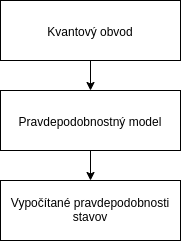
\includegraphics[width=.2\textwidth]{figures/navrh.png} 
	\caption{Konceptuálny návrh programu}
    \label{navrh}
\end{figure}


Pri pohľade na jednoduchý konceptuálny model (obrázok \ref{navrh}) je zrejmé
čo cheme dosiahnuť. Na vstupe je očakávaný kvantový obvod. Samotný program
prebehne tímnto obvodom ako interpreter a zároveň pomerá stavy na daných
miestach v obvode. Nakoniec vypíše výstup v zrozumiteľnej podobe.

\section{Definícia vstupu}

Celý kvantový obvod je možné rozdeliť do vertikálnych blokov alebo levelov.
Každý level obsahuje hradlá, ktorých počet je maximálne rovný počtu 
kvantových bitov, s ktorými daný obvod pracuje. Ak v danom levely nechceme
aplikovať žiadnu operáciu nad bitom, môžme definovať prázdny element.

Čiže kvantový obvod môžeme definovať ako list levelov, pričom level je datová
štruktúra, ktorá obsahuje list hradiel. Okrem hradiel každý level bude
obsahovať prepínač, ktorý siganlizuje či má nastať meranie po aktivácií 
hradiel v leveli.

\section{Pravdepodobnostný model}

\begin{figure}
	\centering 
	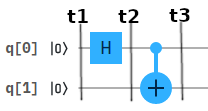
\includegraphics[width=.4\textwidth]{figures/circuit3.png} 
	\caption{Kvantový obvod s previazanými kvantovými bitmi.}
    \label{obvod}
\end{figure}

Pravdepodobnostný model možno vo funkčnosti prirovnať k interpreteru
kvatového obvodu. Tak ako bolo spomenuté v Pravdepodobnostnej analýze 
(kapitola \ref{pravAnalL}) je nutné brať v úvahu previazané a nepreviazané
kvantové bity. Previazanie je možné dosiahnuť hradlom CNOT (respektíve
C\textsuperscript{n}NOT). Našim cieľom nie je vytovoriť dokonalý interpreter,
z tohto dôvodu budeme využívať zjednodušené verzie týchto hradiel. Čo znamená,
že ak kontrólne bity sú v stave \(\ket{1}\) tak cieľový kvantový bit bude 
preklopený hradom \(X\). V inom prípade nenastane zmena v stavoch.


Pravdepodbnostný model si uchováva stavy všetkých kvantových bitova 
v stromovej štruktúre. Pri prechode levelom si uloží nové stavy do listov
tohto stromu. Ak sa v leveli nachádzajú len običajné hradlá, vzniká len
jediný nový list. Rozdiel nastáva pri prechode hradlom CNOT. Je zrejmé, že 
toto hradlo musí rozvetvovať stromovú štruktúru na dva podstromi. Každý z 
podstromov je označený pradvdepodobnosťou, s akou môže nastať daná zmena 
stavov. 

Pri meraní (fiktívnom meraní) sa spočítajú pravdepodobnosti všetkých listov
stromu a výsledky sa uložia do listu. Pre lepšie pochopenie funkčnosti 
programu opíšeme príklad. Majme kvantový obvod, ktorý je definovaný na 
obrázku \ref{obvod}. Na vstupe máme dva kvantové bity v stavoch \(\ket{0}\).
Definujme všetky potrebné datové štruktúry v jazyku Haskell. 

\begin{code}
l1 = Level [E, E] True
l2 = Level [H, E] True
l3 = Level [Cc, Ct] True
c = [l1, l2, l3]
st = StateTree 1 [q0, q0] []
rt = RT st []
\end{code}

Chceme merať v troch časových okamihoch, čo dosiahneme definovaním levelov
l1, l2 a l3. Každý level je označený na meranie pomocou True a využité hradlá
sú nasledovné:
\begin{itemize}
    \item E - prázdne
    \item H - Hadamardovo hradlo
    \item Cc - Kontrólny bit (angl. control bit) hradla CNOT
    \item Ct - Cieľový bit (angl. target bit) hradla CNOT
\end{itemize}

Pre ďalšie spracovanie spojíme levely  do jedného obvodu \(c\). Na ukladanie
stavov slúži stromová štruktúra StateTree. Jej definovaním hovoríme, že
počiatočné stavy sú q0, čo je označenie pre stav \(\ket{0}\). Pravdepodobnosť
dosiahnutia týchto stavov je 1 a zatiaľ neexistujú žiadne podstromi. Štruktúra
RT slúži na ukadanie výsledkov meraní. Spustením pravdepodobnostného modelu
dostaneme výslednú tabuľku typu RT.

\begin{code}
processRT = processCircuit c rt
\end{code}

\begin{figure}
	\centering 
	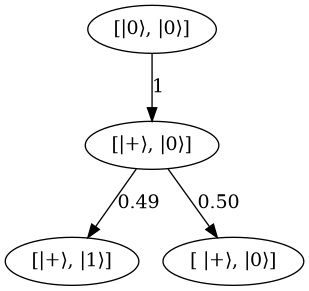
\includegraphics[width=.4\textwidth]{figures/ST.png} 
	\caption{Strom stavov (StateTree) po vykonaní kvantového obvodu.}
    \label{stateTree}
\end{figure}

To ako sa menili stavy kvantových bitov môžeme vidieť na obrázku
\ref{stateTree}. Je zrejmé, že využitím operácie Hadarmardovho hradla nenastane
vetvenie stromu stavov. To isé ale už neplatí pre hradlo CNOT. Nakoľko stav
kontrólneho bitu \(\ket{+}\) má \(50\%\)-tnú šancu skolabovať do stavu 
\(\ket{0}\) ako aj do stavu \(\ket{1}\), tak je prirodzené, že strom stavov 
sa rozvetví a každý podstrom má pravdepodobonsť dosihuntia približne \(0.5\).

Pri výpočte výsledkov je nutné započítať nie len pravdepodobnosti kolabovania
výsledných stavov ale aj pravdepodobnosti dosiahnutia podstromov, v ktorých 
sa dané stavy kvantových bitov nachádzajú. Meriame pravdepodobnosti kolabovania
bitov do stavov \(\ket{0}\) a \(\ket{1}\). Ide o dva stavy takže počet
kombinácií výsledkov je \(2^n\), kde \(n\) je počet kvantových bitov v obvode.
Teda pre dva bity možné kombinácie sú \(\ket{00}, \ket{01}, \ket{10}\) a
\(\ket{11}\). Vypočítajme výsledky pre level l3, čiže vychádzame z listov 
finálneho stromu stavov. Pre prvý list pravdepodobnosť dosiahnutia stavu:

\begin{itemize}
    \item \(\ket{00}\) je \(|\alpha_0\alpha_1|^2 = |\binom{1}{\sqrt{2}} \times
0|^2 = 0\)
    \item \(\ket{01}\) je \(|\alpha_0\beta_1|^2 = |\binom{1}{\sqrt{2}} \times
1|^2 = 0.5\)
    \item \(\ket{10}\) je \(|\beta_0\alpha_1|^2 = |\binom{1}{\sqrt{2}} \times
0|^2 = 0\)
    \item \(\ket{11}\) je \(|\beta_0\beta_0|^2 = |\binom{1}{\sqrt{2}} \times
1|^2 = 0.5\)
\end{itemize}

Pre druhý list obdobne platí to isté. Samozrejme treba započítať aj
pravdepodobnosť vykonania podstromu. Čiže všetky tieto pravdepodobnosti
kolabovania je nutné vynásobiť príslušnými hodnotami. Teda dostávame výsledky:
\begin{itemize}
    \item \(\ket{00}\) dosiahneme s pravdepodobnosťou \(0.25\)
    \item \(\ket{01}\) dosiahneme s pravdepodobnosťou \(0.25\)
    \item \(\ket{10}\) dosiahneme s pravdepodobnosťou \(0.25\)
    \item \(\ket{11}\) dosiahneme s pravdepodobnosťou \(0.25\)
\end{itemize}

% !TEX root = ../thesis.tex

\chapter{Kvantová teleportácia}

Predstavme si situáciu, že chceme na diaľku komunikovať. Chceme poslať
informáciu o stave kvantového bitu. Zaznamenať komplexné číslo úplne presne 
na číslicovom počítači nejde, a teda nemožno poslať niekomu informáciu o 
presnom stave. Takisto platí, že kvantové bity je nemožné kopírovať či
klonovať. Spôsobom akým je možné riešiť tento problém je takzvaná kvantová
teleportácia.

Medzi účastníkov komunikácie sa rozdelí dvojica previazaných bitov. Ak tieto
kvantové bity nemeriame, zachovajú si svoj stav aj previazanie nehľadiac
na fyzickú vzdialenosť medzi nimi. Teda je možné komunikovať aj na diaľku.

Uveďme si všeobecne známy príklad na kvantovú teleportáciu. Povedzme, že 
Bob chce poslať kvantový bit Alici. Najprv je nutné aby obaja vlastnili
pár previazaných kvantových bitov. Ak teraz chce Bob poslať bit Alici, jediné
čo musí spraviť je aplikovať CNOT hradlo na svoj previazaný bit, ktorý bude 
kontrolovaný kvantovým bitom, ktorý chce odoslať. Potom aplikuje Hadamardovo
hradlo na odosielaný bit a pomeria obe bity. Alici odošle informáciu o
stavoch, ktoré kolabovaním dostal. Alica z tejto informácie vie, ako má použiť
hradlá X a Z, tak aby dosiahla rovnaký stav bitu, ktorý povodne vlastnil Bob.

Týmto spôsobom je možné informáciu poslať nakoľko sa jedná o celé čísla.
Takisto nie je porušená veta o kopírovaní ani klonovaní kvantových bitov, 
nakoľko Bob svoj bit stratil.

Ukážme si to na kvantovom obvode. Vytvoríme previazaný pár kvantových bitov
ako na obrázku \ref{tel_c1}. Povedzme, že bit \(q_1\) patrí Bobovi a \(q_2\)
je Alicin.

\begin{figure}[H]
	\centering 
	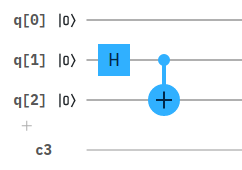
\includegraphics[width=.5\textwidth]{figures/tel_c1.png} 
	\caption{Previazanie kvantových bitov na kvantovú teleportáciu.}
    \label{tel_c1}
\end{figure}

Ako bolo spomenuté, na to aby mohol Bob poslať bit \(q_0\), musí aplikovať
CNOT a následne Hadamardovo hradlo, tak ako na obrázku \ref{tel_c2}.

\begin{figure}[H]
	\centering 
	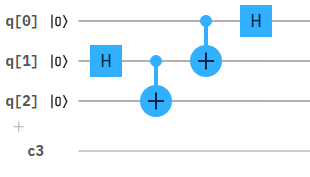
\includegraphics[width=.5\textwidth]{figures/tel_c2.png} 
	\caption{Obvod popisujúci kvantovú teleportáciu.}
    \label{tel_c2}
\end{figure}

Bob pomeria svoje bity a pošle tieto merania Alici. Alica na základe týchto
meraní vie, že ak
\begin{itemize}
    \item[] Bobov bit \(q_0\) nadobudne stav \(1\), aplikuj hradlo \(Z\) na 
            \(q_2\)
    \item[] Bobov bit \(q_1\) nadobudne stav \(1\), aplikuj hradlo \(X\) na 
            \(q_2\)
\end{itemize}

\subsection*{IBM Quantum Experience výsledky}
Dokončime obvod. Povedzme, že posielame stav \(\ket{1}\), preto pridáme 
hradlo \(X\) na začiatok obvodu a plikujeme na \(q_0\). Na koniec pridáme 
podmienené aplikácie hradiel \(Z\) a \(X\). IBM QX podporuje variantu hradla
\(CNOT\), kde namiesto preklopenia \(X\) aplikujeme \(Z\). Výsledný obvod aj
s meraniami je na obrázku \ref{tel_qx_results}.

\begin{figure}
	\centering 
	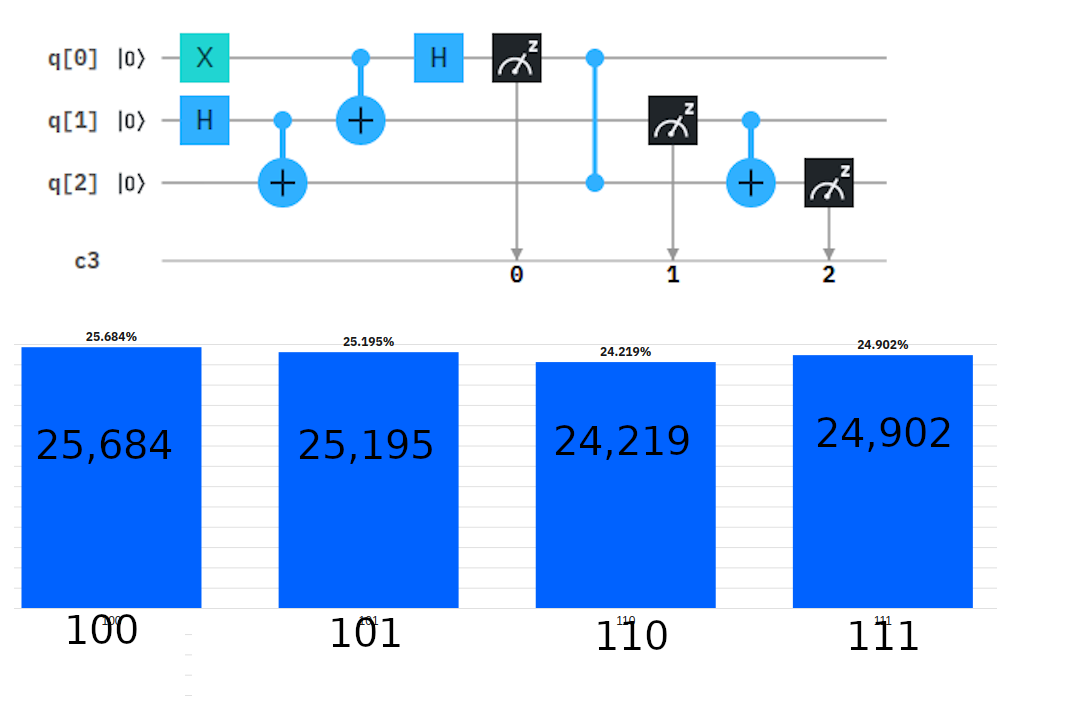
\includegraphics[width=.7\textwidth]{figures/tel_qx_results.png} 
	\caption{Výsledky príkladku kvanovej teleportácie.}
    \label{tel_qx_results}
\end{figure}

Podľa výslekov je jasné, že teleportácia bola úspešná. Najhlavnejší bit 
všetkých výsledkov je \(1\). To znamená, že Alicin kvantový bit vždy nadobudne
taký stav aký mal pôvodne Bob, čo bolo \(\ket{1}\).

\subsection*{Pravdepodobnostný model}
Definujeme kvantový obvod pre program v jazyku Haskell.

\begin{code}
let l1 = Level [E, H, E] True
    l2 = Level [E, Cc, Ct] True
    l3 = Level [Cc, Ct, E] True
    l4 = Level [H, E, E] True
    c = [l1, l2, l3, l4]
    st = StateTree 1 [q1, q0, q0] []
    rt = RT st []
\end{code}
   
Bit \(q_0\) nastavýme na stav \(\ket{1}\), ostatné na \(\ket{0}\). V našom
pravdepodobnostnom modeli nejestvuje možnosť podmienených aplikácií hradiel,
tak si budeme musieť vystačiť s neúplnou teleportáciou.

Fiktívne meranie je nastavené za každým levelom, výsledky meraní su v tabuľke
\ref{tel_results}.

\begin{table}
\centering

\begin{tabular}{|c|c|}
\hline
0.50 & 0.49 \\ 
100 & 110 \\ 
\hline
\end{tabular}

\begin{tabular}{|c|c|c|c|}
\hline
0.25 & 0.249 & 0.25 & 0.25 \\ 
101 & 111 & 100 & 110 \\ 
\hline
\end{tabular}

\begin{tabular}{|c|c|c|c|c|c|c|c|}
\hline
0.25 & 0.249 & 0.0 & 0.0 & 0.25 & 0.25 & 0.0 & 0.0 \\ 
101 & 111 & 101 & 111 & 100 & 110 & 100 & 110 \\ 
\hline
\end{tabular}

\begin{tabular}{|c|c|c|c|c|c|c|c|}
\hline
0.125 & 0.1249 & 0.1249 & 0.1249 & 0.125 & 0.125 & 0.125 & 0.1249 \\ 
001 & 011 & 101 & 111 & 000 & 010 & 100 & 110 \\ 
\hline
\end{tabular}

\caption{\label{tel_results} Výsledky merania experimentu kvantovej
teleportácie pomocou
pravdepodobnostného modelu. Ohraničené riadky vymedzujú výsledky v jednotlivých
 časoch merania. Každá bunka obsahuje pravdepodobnosť dosiahnutia stavu a 
daný stav systému.}
\end{table}

Opäť pripomeňme, že poradie bitov vo výsledkoch z pravdepodobnostného modelu
a výsledkoch IBM QX je opačné. Pozornému oku neunikne, že v niektorých 
prípadoch výsledky po použití hradiel \(X\) a \(Z\) nebudú dávať správny 
výsledok. Je nutné podotknúť, že pravdepodobnostný model nepracuje až tak 
na základe vstupných stavov kvantových bitov v obvode ako na základe
matematikého modelu pravdepodobností dosiahnutia stavov \(\ket{0}\) a 
\(\ket{1}\). Takisto je vydno, že niektoré možnosti sú nedosiahnuteľné.
Teda výsledky pravdepodobnostného modelu sú narozdiel od IBM QX odvodzované od
všeobecných stavov kvantových bitov \(\ket{\psi}\) a vstupné hodnoty stavov
týchto bitov sú použité len na upravednie pravdepodobností do finálnej podoby.

% !TEX root = ../thesis.tex

\chapter{Celkové vyhodnotenie}

V tejto práci sme uviedli spôsob vykonávania a merania kvantových obvodov.
Využitím vedomostí z matematiky a funkcionálneho programovania sme úspešne 
navrhli a implementovali model pre počítanie fiktívnych meraní kvantových
bitov v kvantových obvodoch.

I keď nie je možné porovnávať simulátor kvantového stroje IBM Quantum
Experience s pravdepodobnostným modelom je nutné vyzdvihnúť fakt, že k
výsledkom a teda k predstave ako prebieha kvantový program sa dostaneme 
oveľa rýchlejšie. Na obrázku \ref{expr_time} sú zobrazené výpisy o dokončení
meraní experimentu v IBM QX. Pri experimentoch, ktoré sme vykonávali sme 
robili štyri fiktívne merania. Pre zistenie výsledkov zo simulátora kvantového
stroja, bolo potrebné vykonať jednotlivé merania osobitne a to zabralo relatívne
veľa času. Ako vidíme na obrázku (\ref{expr_time}), vykonanie štyroch 
takýchto meraní trvalo viac ako dve minúty. Kde náš pravdepodobnostný model
vďaka tomu, že nemusí robiť reálne meranie ale len to fiktívne, vracia 
výsledky okamžite. 

\begin{figure}
	\centering 
	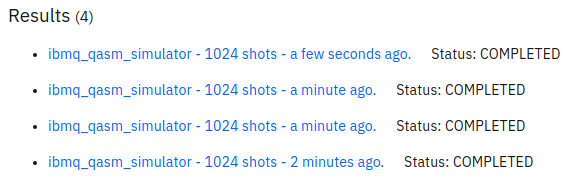
\includegraphics[width=.8\textwidth]{figures/time_expr.png} 
	\caption{Časy dokončení meraní experimetov.}
    \label{expr_time}
\end{figure}


Samozrejme, že ak potrebujeme presné merania, je lepšie použiť kompletný
simulátor. No výhodou nášho riešenia je zobrazenie zmien stavov kvantových
bitov. IBM QX dokáže zobraziť len skolabované výsledky meraní, i keď veľmi
presne, no niekedy je vhodnejšie vedieť stav ešte pred kolabovaním. Náš 
pravdepodobnosný model generuje stromovú štruktúru, v ktorej si zaznamenáva
priebežné stavy kvantových bitov. Získané stromy z našich experimentov sme 
pridali do príloh tejto práce.

Funkčnosť modelu sme otestovali na troch experimetoch. V každom experimente 
sme odvodili vzorce pre výpočet pravdepodobností kolabovania do jednotlivých
stavov pre všetky definované časové okamihy. Uviedli sme výsledky, ktoré 
sú dosiahnuteľné pomocou kvantového stroja IBM Quantum Experience. Nakoniec 
sme pre každý experiment uskutočnili meranie pomocou nášho pravdepodobnostného
modelu.

V neposlednej rade sme preskúmali aj možnosť využitia tohto pravdepodobnostného
modelu aj pri zložitejšom príklade, v ktorom prebiehal kvantový jav zvaný
kvantová teleportácia.


%% !TEX root = ../thesis.tex

\chapter{Meranie jednoduchého kvantového obvodu}

\begin{tikzpicture}[sibling distance=7cm,  every node/.style = {shape=rectangle, rounded corners,    draw, align=center,    top color=white, bottom color=blue!20}]]
  \node[text width=6cm]{ \textbf{1.0:: }[[1.0 :+ 0.0],[0.0 :+ 0.0]],[[1.0 :+ 0.0],[0.0 :+ 0.0]], } [level distance=2cm]
	child { node[text width=6cm]{ \textbf{1.0:: }[[0.7071067811865475 :+ 0.0],[0.7071067811865475 :+ 0.0]],[[1.0 :+ 0.0],[0.0 :+ 0.0]], } [level distance=2cm]
	child { node[text width=6cm] { \textbf{0.4999999999999999:: }[[0.7071067811865475 :+ 0.0],[0.7071067811865475 :+ 0.0]],[[0.0 :+ 0.0],[1.0 :+ 0.0]], } }
	child { node[text width=6cm] { \textbf{0.5000000000000001:: }[[0.7071067811865475 :+ 0.0],[0.7071067811865475 :+ 0.0]],[[1.0 :+ 0.0],[0.0 :+ 0.0]], } } };
\end{tikzpicture}

\begin{tabular}{|c|c|}
\hline
0.5000000000000001 & 0.4999999999999999 \\ 
00 & 10 \\ 
\hline
\end{tabular}

\begin{tabular}{|c|c|c|c|}
\hline
0.25 & 0.2499999999999999 & 0.2500000000000001 & 0.25 \\ 
01 & 11 & 00 & 10 \\ 
\hline
\end{tabular}

\newpage

 \begin{tikzpicture}[sibling distance=7cm,  every node/.style = {shape=rectangle, rounded corners,    draw, align=center,    top color=white, bottom color=blue!20}]]
  \node[text width=6cm]{ \textbf{1.0:: }[[1.0 :+ 0.0],[0.0 :+ 0.0]],[[1.0 :+ 0.0],[0.0 :+ 0.0]], } [level distance=2cm]
	child { node[text width=6cm]{ \textbf{1.0:: }[[0.7071067811865475 :+ 0.0],[0.7071067811865475 :+ 0.0]],[[1.0 :+ 0.0],[0.0 :+ 0.0]], } [level distance=2cm]
	child { node[text width=6cm]{ \textbf{0.4999999999999999:: }[[0.7071067811865475 :+ 0.0],[0.7071067811865475 :+ 0.0]],[[0.0 :+ 0.0],[1.0 :+ 0.0]], } [level distance=2cm]
	child { node[text width=6cm] { \textbf{0.4999999999999999:: }[[0.9999999999999998 :+ 0.0],[0.0 :+ 0.0]],[[0.0 :+ 0.0],[1.0 :+ 0.0]], } } }
	child { node[text width=6cm]{ \textbf{0.5000000000000001:: }[[0.7071067811865475 :+ 0.0],[0.7071067811865475 :+ 0.0]],[[1.0 :+ 0.0],[0.0 :+ 0.0]], } [level distance=2cm]
	child { node[text width=6cm] { \textbf{0.5000000000000001:: }[[0.9999999999999998 :+ 0.0],[0.0 :+ 0.0]],[[1.0 :+ 0.0],[0.0 :+ 0.0]], } } } };
\end{tikzpicture}

\begin{tabular}{|c|c|}
\hline
0.5000000000000001 & 0.4999999999999999 \\ 
00 & 10 \\ 
\hline
\end{tabular}

\begin{tabular}{|c|c|c|c|}
\hline
0.25 & 0.2499999999999999 & 0.2500000000000001 & 0.25 \\ 
01 & 11 & 00 & 10 \\ 
\hline
\end{tabular}

\begin{tabular}{|c|c|}
\hline
0.4999999999999999 & 0.5000000000000001 \\ 
01 & 00 \\ 
\hline
\end{tabular}


%% !TEX root = ../thesis.tex

\chapter{Bezpečnostná analýza}


Pre dosiahnutie robustného riešenia sme museli zvážiť bezpečnostnú stránku programu.
Z tohto dôvodu sme vykonali bezpečnostnú analýzu.
Na vykonanie analýzy sme namodelovali diagram hrozieb pomocou nástroja Microsoft Threat Modeling Tool.
Na obrázku \ref{bez_di} je tento diagram.
Pomocou tohto programu sme veľmi rýchlo odhalili bezpečnostné hrozby, ktoré by mohli ohroziť vykonávanie nášho programu a dáta používateľa.
Ďalej v tejto kapytole popisujeme výstup našej analýzy.

\section{Zhrnutie modelu hrozby}

\begin{figure}[!t] 
	\centering 
	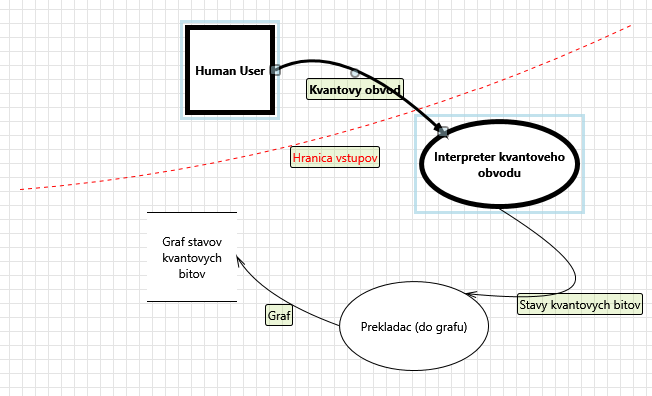
\includegraphics[width=.8\textwidth]{figures/diagram.png} 
	\caption{Diagram modelu hrozieb}
    \label{bez_di}
\end{figure}

\begin{enumerate}

\item \textbf{Spoofing cieľového dátového úložiska Graf stavov kvantovych bitov} \\ 
\textbf{Stav:} migrácia implementovaná \\
\textbf{Priorita:} vysoká
\begin{itemize}

\item[] \textbf{Kategória:} \\
Spoofing je, keď proces alebo entita je niečo iné ako jej nárokovaná identita. Medzi príklady patrí nahradenie procesu, súboru, webovej stránky alebo sieťovej adresy.
\item[] \textbf{Opis:} \\
Graf stavov kvantovych bitov môže útočník spoofovať, a to môže viesť k tomu, že údaje sa zapíšu do cieľa útočníka namiesto grafov kvantovych bitov. Zvážte použitie štandardného autentifikačného mechanizmu na identifikáciu cieľového úložiska údajov.
\item[] \textbf{Odôvodnenie:} \\
Použitie hashov na autentifikáciu.
\end{itemize}

\item \textbf{Potenciálna nadmerná spotreba zdrojov pre Prekladac (do grafu) alebo Graf stavov kvantovych bitov} \\
\textbf{Stav:} Vyžaduje sa vyšetrovanie \\
\textbf{Priorita:} vysoká 

\begin{itemize}
\item[] \textbf{Kategória:} \\
Odopretie služby nastane, keď proces alebo dátové úložisko nie je schopné obsluhovať prichádzajúce žiadosti alebo vykonávať špecifikácie.
\item[] \textbf{Opis:}  \\
Vykonáva prekladac (do grafu) alebo graf stavov kvantovych bitov výslovné kroky na kontrolu spotreby zdrojov? Útoky na spotrebu zdrojov môžu byť ťažko zvládnuteľné a niekedy je rozumné nechať OS robiť svoju prácu. Dávajte pozor, aby vaše žiadosti o zdroje neboli zablokované a aby nevypršali časové limity.
\item[] \textbf{Odôvodnenie:} \\
<neposkytuje sa migrácia>
\end{itemize}

\item \textbf{Podvádzanie externého subjektu - ľudského používateľa} \\
\textbf{Stav:} migrácia implementovaná \\
\textbf{Priorita:} vysoká 

\begin{itemize}
\item[] \textbf{Kategória:} \\
Spoofing je, keď proces alebo entita je niečo iné ako jej nárokovaná identita. Medzi príklady patrí nahradenie procesu, súboru, webovej stránky alebo sieťovej adresy.
\item[] \textbf{Opis:} \\
Ľudský užívateľ môže byť spoofovaný útočníkom a to môže viesť k neoprávnenému prístupu k interpretátoru kvantoveho obvodu. Zvážte použitie štandardného autentifikačného mechanizmu na identifikáciu externej entity.
\item[] \textbf{Odôvodnenie:} \\
Použitie autentifikácie.
\end{itemize}

\item \textbf{Nadväznosť pomocou zosobnenia} \\
\textbf{Stav:} migrácia implementovaná \\
\textbf{Priorita:} vysoká

\begin{itemize}
\item[] \textbf{Kategória:} \\
Subjekt používateľa získava zvýšenú spôsobilosť alebo privilégium využitím chyby implementácie.
\item[] \textbf{Opis:} \\
Interpreter kvantoveho  obvodu môže byť schopný zosobniť kontext ľudského používateľa, aby získal ďalšie privilégiá.
\item[] \textbf{Odôvodnenie:} \\
ACL
\end{itemize}

\item \textbf{Spoofing procesu interpretera kvantoveho obvodu} \\
\textbf{Stav:} migrácia implementovaná \\
\textbf{Priorita:} vysoká

\begin{itemize}
\item[] \textbf{Kategória:} \\
Spoofing je, keď proces alebo entita je niečo iné ako jej nárokovaná identita. Medzi príklady patrí nahradenie procesu, súboru, webovej stránky alebo sieťovej adresy.
\item[] \textbf{Opis:} \\
Interpreter kvantoveho obvodu môže útočník spoofovať, čo môže viesť k poskytovaniu informácií ľudským používateľom. Zvážte použitie štandardného autentifikačného mechanizmu na identifikáciu cieľového procesu.
\item[] \textbf{Odôvodnenie:} \\
Použitie autentifikácie
\end{itemize}

\item \textbf{Potenciálne nedostatočné overenie vstupu pre Interpreter kvantoveho obvodu} \\
\textbf{Stav:} migrácia implementovaná \\
\textbf{Priorita:} vysoká

\begin{itemize}
\item[] \textbf{Kategória:} \\
Manipulácia je akt zmeny bitov. Manipulácia s procesom zahŕňa zmenu bitov v bežiacom procese. Podobne manipulácia s dátovým tokom zahŕňa zmenu bitov na drôte alebo medzi dvoma bežiacimi procesmi.
\item[] \textbf{Opis:} \\
Údajom, ktorý tečie cez Kvantovy obvod, môže útočník zmanipulovať. Môže to viesť k odmietnutiu služobného útoku na tlmočníka kvantového rozsahu alebo k zvýšeniu výsadného privilégia proti tlmočníkovi kvantového množstva alebo k sprístupneniu informácií interpretom kvantového množstva. Opomenutie overiť, či je vstup očakávaný, je hlavnou príčinou veľmi veľkého množstva problémov, ktoré možno zneužiť. Zvážte všetky cesty a spôsob spracovania údajov. Overte správnosť všetkých vstupov pomocou schváleného prístupu na overenie vstupu do zoznamu.
\item[] \textbf{Odôvodnenie:} \\
Validácia vstupu.
\end{itemize}

\item \textbf{Potenciálne odmietnutie údajov Interpretera kvantového obvodu} \\
\textbf{Stav:} migrácia implementovaná \\
\textbf{Priorita:} vysoká

\begin{itemize}
\item[] \textbf{Kategória:} \\
Hrozby odmietnutia zahŕňajú protivníka, ktorý popiera, že sa niečo stalo.
\item[] \textbf{Opis:} \\
Interpreter kvantoveho obvodu tvrdí, že nedostal údaje zo zdroja mimo hranice dôveryhodnosti. Zvážte použitie protokolovania alebo auditu na zaznamenanie zdroja, času a súhrnu prijatých údajov.
\item[] \textbf{Odôvodnenie:} \\
Audit vstupov.
\end{itemize}

\item \textbf{Sniffing toku údajov} \\
\textbf{Stav:} migrácia implementovaná \\
\textbf{Priorita:} vysoká

\begin{itemize}
\item[] \textbf{Kategória:} \\ 
Zverejňovanie informácií nastane, keď ich môže prečítať neoprávnená strana.
\item[] \textbf{Opis:} \\
Údaj, ktorý tečie cez Kvantovy obvod, môže útočník vyvolať. V závislosti od toho, aký typ údajov môže útočník prečítať, možno ho použiť na útok na iné časti systému alebo jednoducho na odhalenie informácií vedúcich k porušeniu súladu. Zvážte šifrovanie toku údajov.
\item[] \textbf{Odôvodnenie:} \\ 
Ručné zadávanie.
\end{itemize}

\item \textbf{Potenciálne zlyhanie procesu alebo zastavenie Interpretera kvantoveho obvodu} \\ 
\textbf{Stav:} migrácia implementovaná \\
\textbf{Priorita:} vysoká

\begin{itemize}
\item[] \textbf{Kategória:} \\
Odopretie služby nastane, keď proces alebo dátové úložisko nie je schopné obsluhovať prichádzajúce žiadosti alebo vykonávať špecifikácie.
\item[] \textbf{Opis:} \\ 
Tlmočník kvantoveho signálu havaruje, zastavuje, ukončuje alebo beží pomaly; vo všetkých prípadoch porušujúcich metriku dostupnosti.
\item[] \textbf{Odôvodnenie:} \\
Využívanie kvót na predchádzanie veľkým vstupom.
\end{itemize}

\item \textbf{Tok údajov Kvantový obvod je potenciálne prerušený} \\
\textbf{Stav:} migrácia implementovaná \\
\textbf{Priorita:} vysoká

\begin{itemize}
\item[] \textbf{Kategória:} \\
Odopretie služby nastane, keď proces alebo dátové úložisko nie je schopné obsluhovať prichádzajúce žiadosti alebo vykonávať špecifikácie.
\item[] \textbf{Opis:} \\
Externý agent preruší údaje tečúce cez hranice dôveryhodnosti v oboch smeroch.
\item[] \textbf{Odôvodnenie:} \\
Validácia používateľa
\end{itemize}

\item \textbf{Interpreter kvantoveho obvodu môže byť predmetom zvýšenia oprávnenia pomocou vzdialeného vykonávania kódu} \\
\textbf{Stav:} migrácia implementovaná \\
\textbf{Priorita:} vysoká

\begin{itemize}
\item[] \textbf{Kategória:} \\
Subjekt používateľa získava zvýšenú spôsobilosť alebo privilégium využitím chyby implementácie.
\item[] \textbf{Opis:} \\ 
Ľudský užívateľ môže byť schopný diaľkovo vykonať kód pre tlmočníka kvantoveho kontroly.
\item[] \textbf{Odôvodnenie:} \\ 
Validácia vstupu.
\end{itemize}

\item \textbf{Vyzdvihnutie zmenou realizačného toku v Interpretore kvantoveho obvodu}  \\
\textbf{Stav:} migrácia implementovaná \\
\textbf{Priorita:} vysoká

\begin{itemize}
\item[] \textbf{Kategória:}  \\
Subjekt používateľa získava zvýšenú spôsobilosť alebo privilégium využitím chyby implementácie.
\item[] \textbf{Opis:} \\ 
Útočník môže preniesť údaje do kvantového interpreta Interpreter, aby zmenil tok vykonávania programu v Interpretore kvantového obvodu podľa výberu útočníka.
\item[] \textbf{Odôvodnenie:} \\ 
Overenie vstupných údajov.
\end{itemize}

\item \textbf{Vyzdvihnutie pomocou zosobnenia} \\ 
\textbf{Stav:} migrácia implementovaná \\
\textbf{Priorita:} vysoká

\begin{itemize}
\item[] \textbf{Kategória:} \\
Subjekt používateľa získava zvýšenú spôsobilosť alebo privilégium využitím chyby implementácie.
\item[] \textbf{Opis:} \\
Prekladač (do grafu) môže byť schopný zosobniť kontext interpretátora kvantovehobvodu, aby získal ďalšie privilégium.
\item[] \textbf{Odôvodnenie:} \\
Nastavenie povolení pre Prekladač (do grafu).
\end{itemize}

\end{enumerate}

\section{Zhrnutie}

Pri analýze sme odhalili 13 hrozieb.
Z hoto sa nám úspešne podarilo vyriešiť 12.
Pomocou tejto metódy sa nám veľmi rýchlo podarilo nájsť a eliminovať bezpečnostné nedostatky nášho programu.


%% !TEX root = ../thesis.tex

\chapter{Celkové vyhodnotenie}

V tejto práci sme uviedli spôsob vykonávania a merania kvantových obvodov.
Využitím vedomostí z matematiky a funkcionálneho programovania sme úspešne 
navrhli a implementovali model pre počítanie fiktívnych meraní kvantových
bitov v kvantových obvodoch.

I keď nie je možné porovnávať simulátor kvantového stroje IBM Quantum
Experience s pravdepodobnostným modelom je nutné vyzdvihnúť fakt, že k
výsledkom a teda k predstave ako prebieha kvantový program sa dostaneme 
oveľa rýchlejšie. Na obrázku \ref{expr_time} sú zobrazené výpisy o dokončení
meraní experimentu v IBM QX. Pri experimentoch, ktoré sme vykonávali sme 
robili štyri fiktívne merania. Pre zistenie výsledkov zo simulátora kvantového
stroja, bolo potrebné vykonať jednotlivé merania osobitne a to zabralo relatívne
veľa času. Ako vidíme na obrázku (\ref{expr_time}), vykonanie štyroch 
takýchto meraní trvalo viac ako dve minúty. Kde náš pravdepodobnostný model
vďaka tomu, že nemusí robiť reálne meranie ale len to fiktívne, vracia 
výsledky okamžite. 

\begin{figure}
	\centering 
	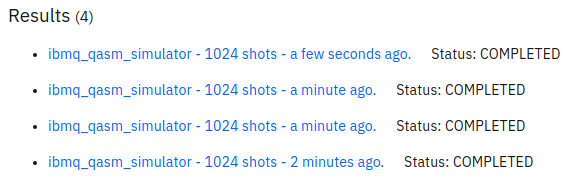
\includegraphics[width=.8\textwidth]{figures/time_expr.png} 
	\caption{Časy dokončení meraní experimetov.}
    \label{expr_time}
\end{figure}


Samozrejme, že ak potrebujeme presné merania, je lepšie použiť kompletný
simulátor. No výhodou nášho riešenia je zobrazenie zmien stavov kvantových
bitov. IBM QX dokáže zobraziť len skolabované výsledky meraní, i keď veľmi
presne, no niekedy je vhodnejšie vedieť stav ešte pred kolabovaním. Náš 
pravdepodobnosný model generuje stromovú štruktúru, v ktorej si zaznamenáva
priebežné stavy kvantových bitov. Získané stromy z našich experimentov sme 
pridali do príloh tejto práce.

Funkčnosť modelu sme otestovali na troch experimetoch. V každom experimente 
sme odvodili vzorce pre výpočet pravdepodobností kolabovania do jednotlivých
stavov pre všetky definované časové okamihy. Uviedli sme výsledky, ktoré 
sú dosiahnuteľné pomocou kvantového stroja IBM Quantum Experience. Nakoniec 
sme pre každý experiment uskutočnili meranie pomocou nášho pravdepodobnostného
modelu.

V neposlednej rade sme preskúmali aj možnosť využitia tohto pravdepodobnostného
modelu aj pri zložitejšom príklade, v ktorom prebiehal kvantový jav zvaný
kvantová teleportácia.

% !TEX root = ../thesis.tex

\chapter{Záver}
Úlohou tejto práce bolo zostaviť programové riešenie problému merania
stavov kvantových bitov počas behu kvantového obvodu. Poskytli sme výstižný
úvod do problematiky kvantových počítačov z pohľadu matematických 
definýcií. Po prečítaní tejto práce by aj laikovy malo byť jasné ako prebieha
kvantový obvod, a na akom princípe fungujú merania bitov.

Ešte pred samotnou implementáciou Haskellovského programu sme sa snažili 
detailne priblížiť na akom matematickom princípre postavíme pravdepodobnostný
model. Analýzu návrhu a proces implementácie tohto pravdepodobnostného modelu
sme rozobrali v jednej z kapitol. Vďaka tomu sme mohli ukázať aj riešenie 
zložitejšieho príkladu kvantového obvodu.

Tak ako sme dokázali pri experimentoch, náš pravdepodobnostný model je 
využiteľný pri tvorbe a analýze kvatnových obvodov. Značne urýchľuje výpočty,
ktoré je nutné vykonávať a odvodzovať pri práci s spomínanými obvodmi.
Poskytuje grafickú podobu zmien stavov, čo len ďalej zjednodušuje pochopenie
práce kvantových počítačov.

Do budúcna by bolo dobré vytvoriť grafické prostredie, ktoré by bolo 
nadstavbov tejto práce. Uľahčilo by to prácu, nakoľko by nebolo nutné poznať
jazyk Haskell pre realizáciu experimentu. Experimenty, ktoré táto práca 
popisuje sú ale dobrým návodom ako tento program využívať. Taktiež obohatenie 
tohto pravdepodobnostného modelu o sofistikovanejší simulátor kvantového stroja
by priniesol presnejšie výsledky, najmä pri obvodoch s previazanými kvantovými
bitmi. V takom prípade by bolo možné úplne nahradiť kvantový simulátor
IBM Quantum Experience, pri návrhu a prvotnom testovaní kvantových obvodoch,
čo by v konečnom dôsledku malo za vpliv rýchlejší rozvoj tejto technológie.


% good linebraking of bibtex url
\setcounter{biburllcpenalty}{7000}
\setcounter{biburlucpenalty}{8000}

%% The bibliography
\phantomsection
\addcontentsline{toc}{chapter}{Literatúra}
\printbibliography[title={Literatúra}]

% List of acronyms
\printglossary[type=\acronymtype,title={\acrlistname}]

%% Appendix
%% !TEX root = ../thesis.tex

\chapter*{Zoznam príloh}
\addcontentsline{toc}{chapter}{Zoznam príloh}

\begin{description}
	\item[Príloha A] Lorem ipsum
    \item[Príloha B] CD médium -- záverečná práca v~elektronickej podobe,
    \item[Príloha C] Používateľská príručka
    \item[Príloha D] Systémová príručka
\end{description}

%\appendix
%\renewcommand\chaptername{Príloha}
%% !TEX root = ../thesis.tex



% zivotopis autora
%\curriculumvitae\protect
%Táto časť\/ je nepovinná. Autor tu môže uviesť\/ svoje biografické
%údaje, údaje o~záujmoch, účasti na~projektoch, účasti na~súťažiach,
%získané ocenenia, zahraničné pobyty na~praxi, domácu prax, publikácie
%a~pod.

\end{document}
